\chapter{Markov Random Fields}
%\label{chap:generative}
\label{chap:mrf}

%%
% !TeX root = graphical.tex

With this chapter, we start a discussion of large-scale statistical models in data science, starting with graphical models (Markov random fields and Bayesian networks) before discussing more recent approaches using, notably, deep learning. Important textbook references for the present chapter include \citet{pearl1988probabilistic, ancona1990random,winkler1995image,lauritzen1996graphical,
cowell07probabilistic,koller2009probabilistic}.

\section{Independence and conditional independence}

\subsection{Definitions}
%The statistical behavior of a large set of random variables can be
%efficiently analyzed from the conditional independence relations they
%have. In this
%section, we review this important concept and discuss its most
%important properties.\\
%
%We assume that $(\Om, \CF, P)$ is a probability space. This means that $\CF$ is a collection of subsets of $\Om$, and $P : \CF\to [0,1]$ is a probability distribution, both $\CF$ and $P$ satisfying the usual probability axioms. A discrete random variable (r.v.) is a mapping $X: \Om \to R_X$, where $R_X:= X(\Om)$ is the set in which $X$ takes its values and is either finite or countable, and $X$ is such that the set (or ``event'')
%\[
%[X=x] = \defset{\om\in \Om: X(\om) = x}
%\]
%belongs to $\CF$, so that $P(X=x)$ is well defined. A real-valued r.v. $X$ is such that the event $X\in I$ belongs to $\CF$ for every real interval $I$, and vector-valued r.v.'s are such that all their coordinates are real-valued r.v.'s. A real-valued r.v. $X$ has a density if  there exists an integrable function $f_X$ defined over $\mR$ such that
%\[
%P(X\in I) = \int_I f_X(x) dx.
%\] 
%
%We will mostly work with discrete random variables in this text.
%
%If $X$ is a discrete random variable and $f:R_X \to \mR$ is a function, the expectation of $f(X)$ is defined by
%\[
%E(f(X)) = \sum_{x\in R_X} f(x) P(X=x).
%\]
%If $R_X\subset \mR$, then one can use $f = \mathrm{identity}$, letting
%\[
%E(X) = \sum_{x\in R_X} x P(X=x).
%\]
%Note that this definition is consistent, in the sense that, if $Y = f(X)$, then $Y$ is also a r.v., and one can check that
%\[
%\sum_{y\in R_Y} y P(Y=y) = \sum_{x\in R_X} f(x) P(X=x)
%\]
%so that the two apparently distinct definitions of $E(Y)$ coincide.
%
%The expectation of real-valued r.v.'s in the non-discrete case, is more difficult to define, and requires measure theory in order to handle  the general case. However, if $X$ has a density, then
%\[
%E(X) = \int_{\mR} x f_X(x) dx
%\]
%provided the integral is convergent.
%\\
%

We consider random variables $X, Y, Z\ldots $, and denote by $\CR_X, \CR_Y, \CR_Z\ldots$ the sets in which they take their values.
We discuss in this section  concepts of independence and conditional independence between random variables. To simplify the exposition, we will work (unless mentioned otherwise) with discrete random variables ($X$ is discrete if $\CR_X$ is finite or countable)\footnote{In the general case, $\CR_X, \CR_Y, \ldots$ are metric spaces with a countable dense subset with $\sigma$-algebras $\boldsymbol{\CS}_X, \boldsymbol{\CS}_Y, \ldots$}.   
We start with a basic definition.
\begin{definition}
\label{def:indep}

Two discrete random variables $X:\Om \to \CR_X$ and $Y:\Om\to \CR_Y$ are independent if and only if
$$
\forall x\in \CR_X, \forall y\in \CR_Y: \myP(X=x, Y=y) = \myP(X=x)\myP(Y=y).
$$
\end{definition}

The general definition for arbitrary r.v.'s is that 
\[
\myE(f(X)g(Y)) = \myE(f(X))\, \myE(g(Y))
\]
 for any pair of (measurable) non-negative functions $f:\CR_X \to [0, +\infty)$ and $g:\CR_Y\to [0, +\infty)$.


%Independence between two variables
%means that $X$ brings no information on $Y$ and vice versa. This can
%be rephrased in terms of conditional expectations and
%distributions. 

One can easily check that $X$ and $Y$ are independent
if and only if, for any non-negative function $g: \CR_Y \to \mR$, one
has
$$
\myE(g(Y)\mid X) = \myE(g(Y)).
$$

 

\begin{notation}
\label{not:ind}
Independence is a
property that involves two variables $X$ and $Y$ and an underlying
probability distribution $\myP$. Independence of $X$ and $Y$ relative to
$\myP$ will be denoted $(X\indp Y)_{\myP}$. However we will only write
$X\indp Y$ when there is no ambiguity on $\myP$.  
\end{notation}


More than independence, the concept of conditional independence will
be fundamental in this chapter. It requires three variables, say
$X,Y,Z$. Returning to the discrete case, one says  that $X$ and $Y$ are conditionally independent
given $Z$ is, for any $x\in \CR_X$, $y\in \CR_Y$ and $z\in \CR_Z$ such that $\myP(Z=z) > 0$,
\begin{equation}
\label{eq:cond.ind.discrete}
\myP(X=x, Y=y\mid Z=z) = \myP(X=x\mid Z=z)\, \myP(Y=y\mid Z=z).
\end{equation}
An equivalent statement is that, for any $z$ such that $\myP(Z=z) \neq 0$,  $X$ and $Y$ are independent when $\myP$
is replaced by the conditional distribution $\myP(\cdot\mid Z=z)$.

In the general case conditional independence means that,  for any pair of non-negative measurable functions $f$ and $g$,
\begin{equation}
\label{eq:cond.ind.gen}
\myE(f(X)g(Y)\mid Z) = \myE(f(X)\mid Z)\,\myE(g(Y)\mid Z).
\end{equation}
From now, we restrict our discussion to discrete random variables.

Multiplying both terms in \cref{eq:cond.ind.discrete} by $\myP(Z=z)^2$, we get the equivalent statement:
$X$ and $Y$ are
conditionally independent given $Z$ if and only if, 
\begin{equation}
\label{eq:cond.ind}
\forall x,y,z: \myP(X=x, Y=y, Z=z)\myP(Z=z) = \myP(X=x, Z=z)\, \myP(Y=y, Z=z).
\end{equation}
Note that the identity is meaningful, and always true, for $\myP(Z=z)=0$, so that this case does not need to be excluded anymore.

Conditional independence  can be interpreted by the statement that $X$ brings no more information on $Y$ than what
is already provided by $Z$: one has
\[
\myP(Y=y\mid X=x, Z=z) = \frac{\myP(Y=y, X=x, Z=z)}{\myP(X=x, Z=z)} = \frac{\myP(Y=y,Z=z)}{\myP(Z=z)}
\]
as directly deduced from \cref{eq:cond.ind}. (This computation being valid as soon as $\myP(X=x, Z=z) > 0$.)




\begin{notation}
\label{not:cond.ind}
To indicate
that $X$ and $Y$ are conditionally independent given $Z$ for the
distribution $\myP$, we will write
$(X\indp Y\mid Z)_{\myP}$ or simply $(X\indp Y\mid Z)$.
\end{notation}
So we have the equivalence:
$$
(X\indp Y\mid Z)_{\myP} \Leftrightarrow \big(\forall z: \myP(Z=z) > 0 \Rightarrow (X\indp Y)_{\myP( \mid Z=z)}\big).
$$

Absolute independence is like ``independence conditional to
no variable'', and we will use the notation $\emp$ for the ``empty'' random
variable that contains no information (for example, a set-valued
random variable that always returns the empty set, or any constant
variable). So we have the tautology
$$
X\indp Y \Leftrightarrow \cind{X}{Y}{\emp}.
$$

Note that, dealing with discrete variables, all previous definitions
automatically extend to groups of variables: for example, if $Z_1$,
$Z_2$ are two discrete variables, so is $Z = (Z_1,Z_2)$ and we
immediately obtain a definition for the conditional independence of $X$ and $Y$ given
$Z_1$ and $Z_2$, denoted $(X\indp Y\mid Z_1,Z_2)$. 

\subsection{Fundamental properties}

Proposition \ref{prop:cind} below lists important properties of conditional
independence that will be used
repeatedly in this chapter. 
 Before stating this proposition, we need
the following definition.

\begin{definition} 
\label{def:posit}
One says that the joint distribution of the random variables $(X_1,
\ldots, X_N)$ is positive if there exists subsets $\tilde R_k\subset \CR_{X_k}$, $k=1, \ldots, N$ such that $\myP(X_k\in \tilde R_k) = 1$ and:
\[
\myP(X_1=x_1, \ldots, X_N=x_N) > 0
\]
if $x_k\in \tilde R_k$, $k=1, \ldots, N$.
\end{definition}
Note that the condition implies $\myP(X_k = x_k) >0$ for all $x_k\in \tilde R_k$, so that $\tilde R_k = \{x_k\in \CR_{X_k}: \myP(X_k=x_k) > 0\}$, i.e., $\tilde R_k$ is the support of $P_{X_k}$. One can interpret the definition as expressing the fact that any conjunction of events for different
$X_k$'s has positive probability, as soon as each of them has positive probability (if all events may occur, then they may occur together). 

Note that the sets $\tilde R_k$ depend on $X_1, \ldots, X_N$. However, if this family of variables is fixed, there is no loss in generality in restricting the space $\CR_{X_k}$ to $\tilde R_k$ and there for assume that $\myP(X_1=x_1, \ldots, X_N=x_N) > 0$ everywhere.

\begin{proposition}
\label{prop:cind}
Let $X,Y,Z$ and $W$ be random variables. The following properties are true.
\begin{enumerate}[label=(CI\arabic*)]
\item Symmetry: $(X\indp Y\mid Z) \Rightarrow (Y\indp X\mid Z)$.
\item Decomposition: $(X\indp (Y, W)\mid Z) \Rightarrow (X\indp Y\mid Z)$.
\item Weak union: $(X\indp (Y,W)\mid Z)  \Rightarrow
(X\indp Y\mid (Z,W))$.
\item Contraction: $\cind{X}{Y}{Z} \text{ and } \cind{X}{W}{(Z,Y)} \Rightarrow
\cind{X}{(Y,W)}{Z}$.
\item Intersection: assume that the joint distribution of $W,Y$
  and $Z$ is positive. Then
\[
\cind{X}{W}{(Z,Y)} \text{ and } \cind{X}{Y}{(Z,W)}
\Rightarrow \cind{X}{(Y,W)}{Z}.
\]
\end{enumerate}
\end{proposition}
\begin{proof}
%(CI1) and (CI2) are obvious consequences of \cref{eq:cond.ind.gen}. For (CI3), we have, using \cref{prop:cond.ind.gen},
%\[
%\myE(f(X)\mid Y, W, Z) = E(f(X) \mid Z)
%
%
%\[
%\myE(f(X) g(Y) h(W, Z)) = \myE(\myE(f(X)\mid W, Y, Z) g(Y) h(W, Z)) = \myE(\myE(f(X)\mid Z) g(Y) h(W, Z)) = \myE(\myE(f(X)\mid Z) \myE(g(Y)\mid W,Z) h(W, Z)) 
%\]
%which proves the result. Note that $\myE(f(X)\mid Z) = \myE(f(X)\mid W,Z)$ by \cref{prop:cond.ind.gen} and (CI2).
%
%For (CI4), applying \cref{prop:cond.ind.gen},
%\[
%\myE(f(X)\mid Y, W, Z) = E(f(X) \mid Z, Y) = E(f(X) \mid Z)
%\]
%which is the desired result.
%
%\[ 
%E(f(X) \mid Y, Z, W) = E(f(X) \mid Z, Y) = E(f(X) \mid Z, W)
%\]  
%

Properties (CI1) and (CI2) are easily deduced from \cref{eq:cond.ind} and left to the reader. To prove
the last three, we will use the notation $P(x), P(x,y)$ etc. instead of
$\myP(X=x), \myP(X=x, Y=y)$, etc. to save space. Identities are assumed to
hold for all $x,y,z,w$ unless stated otherwise. 

For (CI3), we must prove,
according to  \cref{eq:cond.ind}, that
\begin{equation}
\label{eq:ci.1}
P(x,y,z,w) P(z,w) = P(x,z,w) P(y,z,w)
\end{equation}
whenever $P(x,y,z,w) P(z) = P(x,z) P(y,z,w)$. Summing this last
equation over $y$ (or applying (CI2)) yields $P(x,z,w) P(z) = P(x,z)
P(z,w)$. We can note that all terms in \cref{eq:ci.1} vanish when
$P(z) = 0$, so that the identity is true in this case. When $P(z)\neq
0$, the right-hand side of
\cref{eq:ci.1} becomes
\begin{multline*}
(P(x,z) P(z,w)/P(z))P(y,z,w) = (P(x,z)P(y,z,w)/P(z))P(z,w)
=
P(x,y,z,w)P(z,w),
\end{multline*}
using once again the hypothesis. This proves (CI3).

\medskip

For (CI4), the hypotheses are
\[
\begin{cases}
P(x,y,z)P(z) = P(x, z)P(y,z)\\
P(x,y,z,w)P(y,z) = P(x,y,z)P(y,z,w)
\end{cases}
\]
and the conclusion must be
\begin{equation}
  \label{eq:ci.2}
P(x,y,z,w) P(z) = P(x,z)P(y,z,w).  
\end{equation}
Since \cref{eq:ci.2} is true when $P(y,z) = 0$, we assume that this
probability does not vanish and write
\begin{eqnarray*}
P(x,y,z,w)P(z) &=& P(x,y,z)P(z) P(y,z,w)/P(y,z) \\
&=& P(x,z) P(y,z) P(y,z,w)/P(y,z)\\
&=& P(x,z)P(y,z,w)
\end{eqnarray*}
yielding \cref{eq:ci.2}.
  
\medskip

For (CI5), assuming
\begin{equation}
\label{eq:ci5.assum}
\begin{cases}
P(x,y,z,w)P(y,z) = P(x, y,z)P(y,z,w)\\
P(x,y,z,w)P(z,w) = P(x,z,w)P(y,z,w),
\end{cases}
\end{equation}
we want to show that 
$$
P(x,y,z,w)P(z) = P(x,z)P(y,z,w).
$$
Since this identity is  true when any of the events $W=w,
Y=y$ or $Z=z$ has zero probability, we can assume that their
probabilities are positive, which, by assumption, also implies that all
joint probabilities are positive. From the two identities, we get
\[
P(x,y,z,w)/P(y,z,w) = 
P(x, y,z)/P(y,z)  = P(x,z,w)/P(z,w)
\]
This implies
\[
P(x,y,z) = P(y,z) P(x,z,w)/P(z,w)
\]
that we can sum over $y$ to obtain
\[
P(x, z) = P(z)P(x,z,w)/P(z,w)
\]
We therefore get
\[
P(x,y,z,w)/P(y,z,w) = 
 P(x,z,w)/P(z,w) = P(x,z)/P(z),
\]
which is what we wanted.
\end{proof}

A counter-example of (CI5) when the positivity assumption is not satisfied can be built as follows:
let $X$ be a Bernoulli random variable, and let $Y=W=X$. Let $Z$ be any
Bernoulli random variable, independent from $X$. Given $Z$ and $W$,
$X$ and $Y$ are constant and therefore independent. Similarly, given $Z$ and $Y$,
$X$ and $W$ are constant and therefore independent. However,
given $Z$, $X$ and $(Y,W)$ are not independent (they are equal and non
constant).

\subsection{Mutual independence}

Another concept of interest is the mutual (conditional) independence
of more than two random variables. The random variables
$(X_1, \ldots, X_n)$ are mutually conditionally independent given $Z$
if and only if 
$$
\myE(f_1(X_1)\cdots f_n(X_n)\mid Z) = \myE(f_1(X_1)\mid Z)\cdots \myE(f_n(X_n)\mid Z)
$$
for any non-negative measurable functions $f_1, \ldots, f_n$. In terms of discrete
probabilities, this can be written as
\begin{multline*}
P(X_1=x_1, \ldots, X_n=x_n, Z=z) P(Z=z)^{n-1} = \\
P(X_1=x_1, Z=z) \cdots
P(X_n=x_n, Z=z).
\end{multline*}
This will be summarized with the notation
\[
(X_1 \indp \cdots \indp X_n\mid Z).
\]

We have the proposition
\begin{proposition}
\label{prop:mut.indep}
For variables $X_1, \ldots, X_n$ and $Z$, the following properties are equivalent.
\begin{enumerate}[label=(\roman*)]
\item $(X_1 \indp \cdots \indp X_n\mid Z)$;
\item For all $S, T \sub \defset{1, \ldots, n}$ with $S\cap
  T=\emp$, we have:
$\cind{(X_i, i\in S)}{(X_j, j\in T)}{Z}$;
\item For all $s\in \defset{1, \ldots, n}$, we have: $\cind{X_s}{(X_t,
t\neq s)}{Z}$;
\item For all $s\in \defset{2, \ldots, n}$, we have:
$\cind{X_s}{(X_1,\ldots, X_{s-1})}{Z}$.
\end{enumerate}
\end{proposition}
\begin{proof}
It is clear that $\text{(i)} \Ria \cdots \Ria\text{(iv)}$ so it
suffices to prove that $\text{(iv)} \Ria \text{(i)}$. For this, simply
write (applying (iv) repeatedly to $s = n-1, n-2, \ldots$)
\begin{eqnarray*}
\myE(f_1(X_1)\cdots f_n(X_n)\mid Z) &=& \myE(f_1(X_1)\cdots f_{n-1}(X_{n-1})\mid Z)\, \myE(f_n(X_n) \mid Z) \\
&=& \myE(f_1(X_1)\cdots f_{n-2}(X_{n-2})\mid Z)\, \myE(f_{n-1}(X_{n-1}) \mid Z)\\
&& \quad \myE(f_n(X_n) \mid Z) \\
&\vdots &\\ 
&=& \myE(f_1(X_1)\mid Z)\cdots \myE(f_n(X_n)\mid Z).
\end{eqnarray*}
\end{proof}

\subsection{Relation with Information Theory}

Several concepts in information theory are directly related to
independence between random variables. Recall that the (Shannon) entropy of a discrete
probability distribution over a finite set $\CR$
is defined by 
\begin{equation}
\label{eq:entr.1}
\mathcal H(P) = -\sum_{\om\in \CR} \ln P(\om) P(\om).
\end{equation}
Similarly, the entropy of a random variable $X:\Omega \to \CR_X$ is defined by
\begin{equation}
\label{eq:entr.2}
\mathcal H(X) \defeq \mathcal H(P_X) = -\sum_{x\in \CR_X} \ln P(X=x) P(X=x).
\end{equation}
The entropy is always non-negative, and provides a  measure of the
uncertainty associated to $P$. For a given finite set $\CR$,
it is maximal when $P$ is uniform over $\CR$, and minimal (and vanishes) when $P$ is
supported by a single $\om\in \CR$ (i.e. $P(\om) = 1$). 

One defines the entropy of two or more random variables as the entropy
of their joint distribution, so that, for example,
\[
\mathcal H(X,Y) = -\sum_{(x,y)\in \CR_{X}\times \CR_Y} \ln \myP(X=x, Y=y) \myP(X=x, Y=y).
\]

We  have the proposition:
\begin{proposition}
\label{prop:entr.1} For random variables $X_1, \ldots, X_n$, one has
\[
\mathcal H(X_1, \ldots, X_n)\leq \mathcal H(X_1)+\cdots + \mathcal H(X_n)
\]
 with equality
if and only if 
$(X_1, \ldots, X_n)$ are mutually independent. 
\end{proposition}
\begin{proof}
The proof of this proposition uses  properties of the Kullback-Leibler divergence (c.f. \cref{eq:kl.definition}), given by, for two probability distributions
$\pi$ and $\pi'$ on a finite set $\CB$,
$$
\KL(\pi\|\pi') = \sum_{\om\in \CB} \pi(\om) \ln \frac{\pi(\om)}{\pi'(\om)}.
$$
with the convention $\pi\log(\pi/\pi') = 0$ if $\pi=0$ and $=\infty$ if $\pi>0$ and $\pi'=0$. 
%This divergence has several interesting properties, the most important
%for us is that it can be used to assess the proximity between two
%distributions. The following proposition is a standard result that we
%state without proof \cite{cover2012elements}.
%\begin{proposition}
%\label{prop:kl}
%Given two probability distributions $\pi$ and $\pi'$ on $\Om$, we have
%$\KL(\pi\|\pi') \geq 0$ with equality if and only if $\pi=\pi'$.
%\end{proposition}
Returning to  \cref{prop:entr.1}, a straightforward
computation (which is left to the reader) shows that 
\[
\mathcal H(X_1)+\cdots + \mathcal H(X_n) - \mathcal H(X_1, \ldots, X_n) = \KL(\pi\|\pi')
\]
with $\pi(x_1, \ldots, x_n) = \myP(X_1=x_1, \ldots, X_n=x_n)$ and
$\pi'(x_1, \ldots, x_n) = \prod_{k=1}^n \myP(X_k=x_k)$. This makes
 \cref{prop:entr.1} a direct consequence of 
\cref{prop:kl}. 
\end{proof}

The mutual information between two random variables $X$ and $Y$ is
defined by
\begin{equation}
\label{eq:mut.inf}
\mathcal I(X,Y) = \mathcal H(X) + \mathcal H(Y) - \mathcal H(X,Y).
\end{equation}
From  \cref{prop:entr.1}, $\mathcal I(X,Y)$ is nonnegative and
vanishes if and only if $X$ and $Y$ are independent. Also from the
proof of  \cref{prop:entr.1}, $\mathcal I(X,Y)$ is equal to
$\KL(P_{(X,Y)}\|P_X\otimes P_Y)$ where the first probability is the
joint distribution of $X$ and $Y$ and the second one the product of
the marginals of $X$ and $Y$, which coincides with $P_{X,Y}$ if and
only if $X$ and $Y$ are independent.

If $X$ and $Y$ are two random variables, and $y\in \CR_Y$
with $\myP(Y=y) > 0$,
the entropy of the conditional probability $x \mapsto \myP(X=x\mid Y=y)$ is
denoted $\mathcal H(X\mid Y=y)$, and is a function of $y$. The conditional entropy of $X$ given $Y$, denoted $\mathcal H(X\mid Y)$ is the
expectation of $\mathcal H(X\mid Y=y)$ for the distribution of $Y$, i.e.,
\begin{multline*}
\mathcal H(X\mid Y) = \sum_{y\in \CR_Y} \mathcal H(X\mid Y=y) \myP(Y=y)\\
 = -\sum_{x\in
  R_X} \sum_{y\in \CR_Y} \ln \myP(X=x\mid Y=y)
\myP(X=x, Y=y).
\end{multline*}
So, we have (with a straightforward proof)
\begin{proposition}
\label{prop:cond.ent}
Given two random variables $X$ and $Y$, we have
\begin{eqnarray}
\label{eq:cond.ent}
\mathcal H(X\mid Y) &=& -E_{X,Y}(\ln \myP(X=\cdot \mid Y=\cdot))\\
\nonumber
&=& \mathcal H(X,Y) - \mathcal H(Y)
\end{eqnarray}
\end{proposition}
This proposition also immediately  yields:
\begin{equation}
\label{eq:cond.ind.mut}
\mathcal I(X,Y) = \mathcal H(X) - \mathcal H(X\mid Y) = \mathcal H(Y) - \mathcal H(Y\mid X).
\end{equation}
The identity $\mathcal H(X,Y) = \mathcal H(X\mid Y) + \mathcal H(Y)$ that is deduced from
\cref{eq:cond.ent} can be generalized to more than two random
variables (the proof being left to the reader), yielding, if $X_1,
\ldots, X_n$ are random variables:
\begin{equation}
\label{eq:data.proc.eq}
\mathcal H(X_1, \ldots, X_n) = \sum_{k=1}^n \mathcal H(X_k\mid X_1, \ldots, X_{k-1}).
\end{equation}

If $Z$ is an additional random variable, the following identity is
obtained by applying the previous one to conditional distributions
given $Z=z$ and taking averages over $z$:
\begin{equation}
\label{eq:data.proc.eq.2}
\mathcal H(X_1, \ldots, X_n\mid Z) = \sum_{k=1}^n \mathcal H(X_k\mid X_1, \ldots, X_{k-1}, Z).
\end{equation}\\


The following proposition characterizes conditional independence in
terms of entropy.
\begin{proposition}
\label{prop:cond.ind.ent}
Let $X,Y$ and $Z$ be three random variables. The following statements
are equivalent.
\begin{enumerate}[label=(\roman*)]
\item $X$ and $Y$ are conditionally independent given $Z$.
\item $\mathcal H(X,Y\mid Z) = \mathcal H(X\mid Z) + \mathcal H(Y\mid Z)$
\item $\mathcal H(X\mid Y,Z) = \mathcal H(X\mid Y)$
\end{enumerate} 
Moreover, when (i) to (iii) are satisfied, we have:
\begin{itemize}
\item[(iv)] $\mathcal I(X,Y) \leq \min(\mathcal I(X,Z), \mathcal I(Y,Z))$.
\end{itemize}
\end{proposition}
\begin{proof}
From  \cref{prop:entr.1}, we have, for any three random
variables $X,Y,Z$, and any $z$ such that $P(Z=z) >0$,
\[
\mathcal H(X,Y\mid Z=z) \leq \mathcal H(X\mid Z=z) + \mathcal H(Y\mid Z=z).
\]
Taking expectations on both sides implies the important inequality
\begin{equation}
\label{eq:cond.ind.ineq}
\mathcal H(X,Y\mid Z) \leq \mathcal H(X\mid Z) + \mathcal H(Y\mid Z)
\end{equation}
and equality occurs if and only if $\myP(X=x, Y=y\mid Z=z) = \myP(X=x\mid Z=z)
\myP(Y=y\mid Z=z)$ whenever $\myP(Z=z)>0$, that is, if and only if $X$ and $Y$
are conditionally independent given $Z$. This proves that (i) and (ii)
are equivalent. The fact that (ii) and (iii) are equivalent comes from
\cref{eq:data.proc.eq.2}, which gives, for any three random variables
\begin{equation}
\label{eq:data.proc.eq.3}
\mathcal H(X, Y\mid Z) = \mathcal H(X\mid Y,Z) + \mathcal H(Y\mid Z).
\end{equation}

To prove that (i)-(iii) implies (iv), we note that
\cref{eq:cond.ind.ineq} and \cref{eq:data.proc.eq.3} imply that, for
any three random variables:
\[
\mathcal H(X\mid Y,Z) \leq \mathcal H(X\mid Y).
\]
If $X$ and $Y$ are conditionally independent given $Z$, then the right-hand side is equal to $\mathcal H(X\mid Z)$ and this yields
\[
\mathcal I(X,Y) = \mathcal H(X) - \mathcal H(X\mid Y) \leq \mathcal H(X) - \mathcal H(X\mid Z) = \mathcal I(X,Z).
\]
By symmetry, we must also have $\mathcal I(X,Y) \leq \mathcal I(Y,Z)$ so that (iv) is
true. 
\end{proof}
Statement (iv) is often called the data-processing inequality, and has
been used to infer conditional independence within gene networks
\cite{margolin2006}.

\section{Models on undirected graphs}
\label{sec:random.fields}
\subsection{Graphical representation of conditional independence}
%\subsection{Definitions}
An undirected graph is a
collection of vertexes and edges, in which edges link pairs of  vertexes
without order. Edges can therefore be identified to {\em subsets} of cardinality two
of the set of vertexes, $V$. This yields the definition:
\begin{definition}
\label{def:undir.grph}
An undirected graph $G$ is a pair $G = (V,E)$ where $V$ is a finite
set of vertexes and elements $e \in E$ are subsets $e=\{s,t\} \sub V$.
\end{definition}
Note that edges in undirected graphs are defined as sets, i.e.,
unordered pairs, which are delimited with braces in these notes. Later
on, we will use parentheses to represent ordered pairs, $(s,t)\neq
(t,s)$. We will write $s\sim_G t$, or simply $s\sim t$ to indicate
that $s$ and $t$ are connected by an edge in $G$ (we also say that $s$
and $t$ are neighbors in $G$).

\begin{definition}
\label{def:path.undir}

A path in an undirected graph $G=(V,E)$ is a finite sequence $(s_0, \ldots,
s_N)$ of vertexes such that $s_{k-1}\sim s_k \in E$. (A sequence,
$(s_0)$, of length 1 is also a path by extension.)


We say that $s$ and $t$ are connected by a path if either $s=t$ or
there exists a path $(s_0, \ldots,
s_N)$ such that $s_0=s$ and $s_N=t$.

A subset $S\sub G$ is connected if any pair of elements in $S$ can be
connected by a path.

A subset $T\sub G$ separates two other subsets $S$ and $S'$ if all
paths between $S$ and $S'$ must  pass in $T$. We will write
$\cind{S}{S'}{T}$ in such a case. 

%A subset $T\sub G$ separates two other subsets $S$ and $S'$ if, for
%any path $(s_0\in S, s_1, \ldots, s_{N-1}, s_N\in S')$
%between $S$ and $S'$, there exists $k\in\defset{1, \ldots, N-1}$
%with $s_k\in T$ (we will say that the path passes strictly in $T$). We will write
%$\cind{S}{S'}{T}$ in such a case. 

\end{definition}

One of the goals of this chapter is to relate the notion of
conditional independence within a set of variables to separation in a
suitably chosen undirected graph with vertexes in one-to-one
correspondence with the variables. This will also justifies the similarity of
notation  used for separation and conditional independence.

We have the following simple fact:
\begin{lemma}
\label{lem:simple.1}
Let $G=(V,E)$ be an undirected graph, and $S,S',T\sub V$. Then
\[
\cind{S}{S'}{T} \Ria S\cap S' \sub T.
\]
\end{lemma}
Indeed, if $\cind{S}{S'}{T}$ and $s_0 \in S\cap
S'$, the path $(s_0)$ links $S$ and $S'$ and therefore must pass in
$T$. 

 \Cref{prop:cind} translates into similar
properties for separation:
\begin{proposition}
\label{prop:cind.2}
Let $(V, E)$ be an undirected graph and $S,T,U,R$ be subsets
of $V$. The following properties hold
\begin{enumerate}[label=(\roman*)]
\item $(S\indp T|U) \Leftrightarrow (T\indp S|U)$.
\item $(S\indp T\cup R|U) \Rightarrow (S\indp T|U)$.
\item $(S\indp T\cup R|U)  \Rightarrow
(S\indp T| U\cup R)$.
\item $\cind{S}{T}{U} \text{ and } \cind{S}{R}{U\cup T} \Leftrightarrow
\cind{S}{T\cup R}{U}$.
\item $U\cap R = \emp, \cind{S}{R}{U\cup T} \text{ and } \cind{S}{U}{T\cup R}
\Rightarrow \cind{S}{U\cup R}{T}$. 
\end{enumerate}
\end{proposition}
\begin{proof}
(i) is obvious, and for (ii) (and (iii)), if any path between $S$ and $T\cup R$
must pass by $U$, the same is obviously true for a path between $S$
and $T$. 

For the $\Rightarrow$ part of (iv), if a path links $S$ and
$T\cup R$, then it either links $S$ and $T$ and must pass through $U$
by the first assumption, or link $S$ and $R$ and therefore pass through
$U$ or $T$ by the second assumption. But if the path passes through
$T$, it must also pass through $U$ before by the first assumption. In
all cases, the path passes through $U$. The $\Leftarrow$ part of (iv)
is obvious.

Finally, consider (v) and take a path between two distinct elements in
$S$ and $U\cup R$. Consider the first time the path hits $U$ or $R$,
and assumes that it hits $U$ (the other case being treated similarly
by symmetry). Notice that the path cannot hit both $U$ and $R$ at the
same point since $U\cap R = \emp$. From the assumptions, the path must hit
$T\cup R$ before passing by $U$, and the intersection
cannot be  in $R$, so it is in $T$,
which is the conclusion we wanted.
\end{proof}


To make a connection between separation in graphs and conditional
independence between random variables, we consider a graph $G=(V,E)$
and a family of random variables $(\pe X s, s\in V)$ indexed by $V$. Each variable is assumed to take values in a set $F_s = \CR_{\pe X s}$. The collection of values taken by the random variables will be called configurations, and the sets $F_s, s\in V$ are called the state spaces.

Letting $\mathbb F$ denote the collection $(F_s, s\in V)$, we will denote the set of such configurations as $\CF(V, \mathbb F)$. Then $\mathbb F$ is clear from the context, we will just write $\CF(V)$. If $S \subset V$ and $x\in \CF(V, \mathbb F)$, the restriction of $x$ to $S$ is denoted $\pe x S = (\pe x s, s\in S)$. The set formed by those restrictions will be denoted $\CF(S, \mathbb F)$ (or just $\CF(S)$).

\begin{remark}
\label{rem:configurations}
Some care needs to be given to the definition of the space of configurations, to avoid ambiguities when two sets $F_s$ coincide. The configuration $x = (\pe x s, s\in V)$ should be understood, in an emphatic way, as the collection $\hat x = ((s,\pe x s), s\in V)$, which makes explicit the fact that $\pe x s$ is the value observed at vertex $s$. Similarly the emphatic notation for  $\pe x S \in \CF(V, \mathbb F)$ is $\pe {\hat x} S = ((s,\pe x s), s\in S)$. 

In the following, we will not use the emphatic notation to avoid overly heavy expressions, but its relevance should be clear with the following simple example. Take $V = \{1, 2, 3\}$ and $F_1 = F_2 = F_3 = \{0, 1\}$. Let $\pe x 1 = 0$, $\pe x 2 = 0$ and $\pe x 3 = 1$. Then the sub-configurations $\pe x {\{1,3\}}$ and $\pe x {\{2,3\}}$ both corresponds to values $(0,1)$, but we consider them as distinct. In the same spirit, $\pe x 1 = \pe x2$, but $\pe x {\{1\}} \neq \pe x{\{2\}}$
\end{remark}


If $S, T\subset V$ with $S\cap T=\emptyset$, $\pe x S\in \CF(S, \mathbb F)$, $\pe y T\in \CF(T, \mathbb F)$, we will denote their concatenation by 
$\pe x S \wedge \pe y T$, which is the configuration $z = (z_s, s\in S\cup T)\in \CF(T\cup S, \mathbb F)$ such that $\pe z s=\pe x s$ if $s\in S$ and $\pe z s=\pe y s$ if $s\in T$.



We define a {\em random field} over $V$ as a random configuration $X:\Omega \to \CF(V,  \mathbb F)$, that we will denote for short $X = (\pe X s, s\in V)$. If $S\subset V$, the restriction $\pe X S$ will also be denoted $(\pe X s, s\in
S)$. 
  
  
  
We can now write the definition: 
\begin{definition}
\label{def:cond.grph}
Let $G = (V,E)$ be an undirected graph and  $X = (\pe X s, s\in V)$ a
random field over $V$. We say that $X$ is Markov (or
has the Markov property) relative to  $G$ (or is $G$-Markov, or is a
Markov random field on $G$) if and only if, for all $S, T, U \subset V$:
\begin{equation}
\label{eq:cond.grph}
\cind{S}{T}{U} \Rightarrow \cind{\pe X S}{\pe X T}{\pe X U}.
\end{equation}
\end{definition}
Letting the observation over an empty set $S$ be empty, i.e., $X_\emp =
\emp$, this definition includes the statement that, if $S$ and $T$ are
disconnected (i.e., there is no path between them: they are
separated by the empty set), then $\cind{\pe XS}{\pe XT}{\emp}$: $\pe XS$
and $\pe XT$ are independent. 

We will say that a probability distribution $\pi$ on $\CF(V)$ is $G$-Markov if its associated canonical random field $X = (\pe Xs, s\in V)$ defined on $\tilde \Omega = \CF(V)$ by $\pe X s (x) = \pe x s$ is  $G$-Markov.


\subsection{Reduction of the Markov property}

We now proceed, in a series of steps, to a simplification of
 \cref{def:cond.grph} in order to obtain a minimal number of conditional
independence statements. Note that, in its current form, 
\cref{def:cond.grph} requires to check \cref{eq:cond.grph} for any
three subsets of $V$, which provides a huge number of conditions. Fortunately, as we will see, these conditions are not independent, and checking a much smaller number of them will ensure that all of them are true. 

The first step for our reduction is provided by the following lemma.
\begin{lemma}
\label{lem:int.emp}
Let $G = (V,E)$ be an undirected graph and  $X = (X_s, s\in V)$ a
set of random variables indexed by $V$. Then $X$ is $G$-Markov if and
only if, for $S,T,U\sub V$,
\begin{equation}
\label{eq:cond.grph.lem}
S\cap U = T\cap U=\emp \text{ and }\cind{S}{T}{U} \Rightarrow \cind{\pe X S}{\pe X T}{\pe X U}.
\end{equation}
\end{lemma}
\begin{proof}
Assume that \cref{eq:cond.grph.lem} is true, and take any $S,T,U$ with $\cind{S}{T}{U}$.
Let
$A = S\cap U$, $B = T\cap U$ and $C = A\cup B$. Partition $S$ in $S= S_1\cup
A$, $T$ in $T_1\cup B$ and $U$ in $U_1\cup C$. From 
$\cind{S}{T}{U}$, we get $\cind{S_1}{T_1}{U}$. Since $S_1\cap U = T_1\cap
U = \emp$, this implies $\cind{\pe X {S_1}}{\pe X {T_1}}{\pe X U}$. But this implies
$\cind{(\pe X {S_1}, \pe X A)}{(\pe X {T_1}, \pe X B)}{\pe X U}$. Indeed, this property
requires
\begin{multline*}
P_X(\pe x {S_1}\wedge \pe x A\wedge \pe x {T_1}\wedge \pe x B\wedge \pe x {U_1}\wedge \pe y C) P^X(\pe x {U_1}\wedge \pe y C) \\
=  P_X(\pe x {S_1}\wedge \pe x A\wedge \pe x {U_1}\wedge \pe y C)P_X(\pe x {T_1}\wedge \pe x B\wedge \pe x {U_1}\wedge \pe y C)
\end{multline*}
If the configurations $\pe x A, \pe x B, \pe y C$ are not consistent (i.e.,
$\pe x t\neq \pe y t$ for some $t\in C$), then both sides vanish. So we can
assume $\pe x C = \pe y C$ and remove $\pe x A$ and $\pe x B$ from the expression,
since they are redundant. The resulting identity is true since it exactly
states that  $\cind{\pe X {S_1}}{\pe X {T_1}}{\pe X U}$.
\end{proof}

Define the set of neighbors of $s\in V$ (relative to the graph $G$) as
the set of $t\neq s$ such that $\{s,t\}\in E$ and denote this set by
$\mathcal V_s$. For $S\sub V$ define also
$$
\mathcal V_S = S^c\cap \bigcup_{s\in S} \mathcal V_s 
$$
which is the set of neighbors of all vertexes in $S$ that do not belong to
$S$. (Here $S^c$ denotes the complementary set of $S$, $S^c = V\setminus
S$.) Finally, let $\mathcal W_S$ denote the vertexes that are ``remote''
from $S$, $\CW_S = (S\cup \CV_S)^c$.

We have the following important reduction of the condition in  \cref{def:cond.grph}.
\begin{proposition}
\label{prop:mark.prop}
$X$ is Markov relative to $G$ if and only if, for any $S\sub V$,
\begin{equation}
\label{eq:mark.prop}
\cind{\pe X S}{\pe X {\CW_S}}{\pe X {\mathcal V_S}}.
\end{equation}
\end{proposition}
This says that 
$$
\myP(\pe X S = \pe x S \mid \pe X {S^c} = \pe x {S^c})
$$
only depends (when defined) on variables $\pe x t$ for $t\in S\cup \mathcal V_S$. 

\begin{proof} First note that $\cind{S}{\CW_S}{\mathcal V_S}$ is
  always true, since any
path reaching $S$ from $S^c$ must pass through $\mathcal V_S$. This immediately
proves the ``only if'' part of the proposition.

Consider now the ``if'' part. Take $S,T,U$ such that
$\cind{S}{T}{U}$. We want to prove that $\cind{X_S}{X_T}{X_U}$. According to
 \cref{lem:int.emp}, we can assume, without loss of generality, that
$S\cap U = T\cap U = \emp$.

Define $R$ as the set of vertexes $v$
in $V$ such that there exists a path between $S$ and $v$
that
does not pass in $U$. Then:
\begin{enumerate}[label=\arabic*.]
\item $S\sub R$: the path $(s)$ for $s\in S$ does
not pass in $U$ since $S\cap U=\emp$.
\item $U\cap R=\emp$ by definition. 
\item $\CV_R\sub U$: assume that there exists a
point $r$ in $\CV_R$ which is not in $U$. Then $r$ has a neighbor,
say $r'$ in $R$. By definition of $R$, there exists a path from $S$ to
$r'$ that does not hit $U$, and this path can obviously be extended by
adding $r$ at the end to obtain a path that still does not hit
$U$. But this implies that $r\in R$, which contradicts the fact that $\CV_R\cap
R=\emp$. 
\item $T\cap (R\cup \CV_R) = \emp$: if $t\in T$, then $t\not\in R$ from
$\cind{S}{T}{U}$ and $t\not \in \CV_R$ from $T\cap U=\emp$. 
\end{enumerate}

\begin{figure}[h]
\begin{center}

\includegraphics[width=.5\textwidth]{prop8.png}
\caption{\label{fig:prop8}See proof of 
  \cref{prop:mark.prop} for details}
\end{center}
\end{figure}

We can then
write (each decomposition being a partition, implicitly defining the sets $A$,
$B$ and $C$, see Fig. \ref{fig:prop8})
$R = S\cup A$, $U = \CV_R\cup C$, $(R\cup\CV_R)^c = T\cup C\cup B$,
and from $\cind{\pe X R}{\pe X{\CW_R}}{\pe X{\CV_R}}$, we get
$$
\cind{(\pe X S,\pe X A)}{(\pe X T,\pe  X C, \pe X B)}{\pe X {\CV_R}}
$$
which implies
$$
\cind{(\pe X S,\pe X A)}{(\pe X T, \pe X B)}{\pe X {U}}
$$
by (CI3), which finally implies $\cind{\pe X S}{\pe X T}{\pe X U}$ by (CI2).
\end{proof}



For positive probabilities, it suffices to consider singletons in  \cref{prop:mark.prop}.
\begin{proposition}
\label{prop:mark.prop.2}
If the joint distribution of $(\pe X s, s\in V)$ is positive and, for any $s\in V$,
\begin{equation}
\label{eq:mark.prop.2}
\cind{\pe X s}{\pe X {\CW_s}}{\pe X {\mathcal V_s}},
\end{equation}
then
$X$ is Markov relative to $G$. The converse statement is true
without the positivity assumption.
\end{proposition}
\begin{proof}
It suffices to prove that,  if \cref{eq:mark.prop} is true for $S$ and $T\sub V$, with $T\cap S =
\emp$, it is also true for $S\cup
T$. The result will then follow by induction. 
%Using this, we can extend the property, true for singletons in
% \cref{prop:mark.prop.2}, to any subset of $V$.

So, let $U = \mathcal V_{S\cup T}$ and $R = \mathcal W_{S\cup T} = V \setminus (S\cup T\cup
U)$. Then, we have
$$\cind{\pe X S}{\pe X {\mathcal W_S}}{\pe X {\mathcal V_{S}}} \Ria
\cind{\pe X S}{\pe X R}{(\pe X U, \pe X T)}
$$
because $R\sub \mathcal \CW_S$ (if $s\in \mathcal V_S$, then it is
either in $U$ or in $T$ and therefore cannot be in $R$). Similarly, 
$\cind{\pe X T}{\pe X R}{(\pe X U, \pe X S)}$, and (CI5) (for which we need $P$ positive) now
implies $\cind{(\pe X T, \pe X S)}{\pe X R}{\pe X U}$.
\end{proof}
To see that the positivity assumption is needed, consider the following
example with six variables $\pe X 1, \ldots, \pe X 6$, and a graph linking
consecutive integers and closing with an edge between 1 and
6. Assume that $\pe X 1 = \pe X 2=\pe X 4= \pe X 5$, and that $\pe X 1, \pe X 3$ and $\pe X 6$ are
independent. Then  \cref{eq:mark.prop.2}
is true, since, for $k=1,2,4,5$, $\pe X k$ is constant given its
neighbors, and $\pe X 3$ (resp. $\pe X 6$) is independent of the rest of the
variables. But $(\pe X 1, \pe X 2)$ is not independent of $(\pe X 4,\pe X 5)$ given
the neighbors $\pe X 3, \pe X 6$.

Finally, another statement equivalent to 
\cref{prop:mark.prop.2} is the following:
\begin{proposition}
\label{prop:mark.prop.3}
If the joint distribution of $(\pe X s, s\in V)$ is positive and, for any $s,t\in V$,
$$
s\not \sim_G t \Ria \cind{\pe X s}{\pe X t}{\pe X {V\setm \{s,t\}}},
$$
then
$X$ is Markov relative to $G$. The converse statement is true
without the positivity assumption.
\end{proposition}
\begin{proof}
Fix $s\in V$ and assume that 
$\cind{\pe X s}{\pe X R}{\pe X {V\setm R}}$ for any $R\sub \CW_s$ with cardinality
at most $k$ (the statement is true for $k=1$ by assumption). Consider
a set $\tilde R\sub \CW_s$ of cardinality $k+1$, that we decompose into
$R\cup\{t\}$ for some $t\in\tilde R$. We have
$\cind{\pe X s}{\pe X t}{\pe X {V\setm\tilde R}, X_R}$ from the initial hypothesis
and 
$\cind{\pe X s}{\pe X R}{\pe X {V\setm\tilde R}, X_t}$ from the induction
hypothesis. Using property (CI5), this yields 
$\cind{\pe X s}{\pe X {\tilde R}}{\pe X {V\setm\tilde R}}$. This proves the
proposition by induction.
\end{proof}

\begin{remark}
It is obvious from the definition of a $G$-Markov process that, if
$X$ is Markov for a graph $G=(V, E)$, it is automatically Markov
for any richer graph, i.e., any graph $\tilde G=(V, \tilde E)$ with
$E\sub \tilde E$. This is because separation in $\tilde G$ implies
separation in $G$. Moreover, any $X$ is $G$-Markov for the {\em complete graph} on $V$, for which $s\sim
t$ for all $s\neq t\in V$. This is because no pair of sets can be
separated in a complete graph. 

Any graph with respect to which $X$ is Markov must be richer than the 
graph $G_X = (V,E_X)$ defined by $s\not\sim_{G_X} t$ if and only
$\cind{\pe X s}{\pe X t}{\pe X {\{s,t\}^c}}$. This is true because, for
any graph $G$ for which $X$ is Markov, we have 
$$
s\not\sim_{G} t\Ria \cind{\pe X s}{\pe X t}{\pe X {\{s,t\}^c}} \Ria
s\not\sim_{G_X} t.
$$
Interestingly,  \cref{prop:mark.prop.3} states that $X$ is
$G_X$-Markov as soon as its joint distribution is positive. This
implies that $G_X$ is the minimal graph over which $X$ is Markov in
this case. 
\end{remark}

\subsection{Restricted graph and partial evidence}
Assume that some variables $\pe X T = (\pe X t, t\in T)$ (with $T\sub V$) have been observed,
with observed values $\pe x T = (\pe x t, t\in T)$. One would like to use this
 partial evidence to get additional information on the
remaining variables, $\pe X S$ where $S = V \setm T$. From the
probabilistic point of view, this means computing the conditional
distribution of $\pe X S$ given $\pe X T=\pe x T$.

One important property of $G$-Markov models is that the Markov
property is essentially conserved when passing to conditional
distributions. We introduce for this the following definitions.
\begin{definition}
\label{def:subg}
If $G = (V,E)$ is an undirected graph, a subgraph of $G$ is a graph
$G'=(V',E')$ with $V'\sub V$ and $E'\sub E$.

If $S\sub V$, the {\em restricted graph}, $G_S$, of $G$ to $S$ is defined by
\begin{equation}
\label{eq:rest.grph}
G_S = (S, E_S) \text{ with } E_S = \defset{e = \{s,t\}: s,t\in S \text {
and } e \in E}.
\end{equation}
\end{definition}

We have the following proposition.
\begin{proposition}
\label{prop:cond.dist.grph}
Let $G = (V,E)$ be an undirected graph and $X$ be $G$-Markov. Let
$S\sub V$ and $T = S^c$. Given a partial evidence $\pe x T$ such that
$P(\pe X T=\pe x T)>0$,  $\pe X S$, conditionally to $\pe X T=\pe x T$, is
$G_S$-Markov.
\end{proposition}
\begin{proof}
The proof is straightforward once it is noticed that 
\[
\cind{A}{B}{C}_{G_S} \Ria \cind{A}{B}{C\cup T}_G
\]
so that
\begin{eqnarray*}
\cind{A}{B}{C}_{G_S} &\Ria& \cind{\pe X A}{\pe X B}{\pe X C, \pe X T}_P\\
&\Ria& \cind{\pe X A}{\pe X B}{\pe X C}_{P(\cdot\mid \pe X T=\pe x T)}
\end{eqnarray*}
\end{proof}

\subsection{Marginal distributions}
The effect of taking marginal distributions for a $G$-Markov model is,
unfortunately, not as much a mild operation as computing conditional
distributions, in the sense that the conditional independence structure
of the marginal distribution may be much more complex than the original one.

Let $G = (V, E)$ be an undirected graph, and let $S$ be a subset of
$V$. Define the graph $G^S = (S, E^S)$ by $\{s, t\}\in E^S$ if and
only if $\{s, t\}\in E$ or there exist $u, u'\in S^c$ such that
$\{s,u\} \in E$, $\{t, u'\}\in E$ and $u$ and $u'$ are connected by a
path in $S^c$. In other terms $E^S$ links all $s,t\in S$ that can be
connected by a path, all but the extremities of which are included in
$S^c$.
  With this notation, the
following proposition holds.

\begin{proposition}
\label{prop:margin}
Let $G = (V, E)$ be an undirected graph, and $S\sub V$. Assume that
$X = (\pe X s, s\in V) $ is a family of random variables which is 
$G$-Markov. Then $\pe X S = (\pe x s, s\in S)$ is $G^S$-Markov.
\end{proposition}
\begin{proof}
It suffices to prove that, for $A,B,C\sub S$,
\[
\cind{A}{B}{C}_{G^S} \Ria \cind{A}{B}{C}_G.
\]
So, assume that $A$ and $B$ are
separated by $C$ in $G^S$. If a path connects $A$ and $B$ in
$G$, we can, by definition of $E^S$, remove from this path any portion
that passes in $S^c$ and obtain a valid path in $G^S$. By assumption,
this path must pass in $C$, and therefore so does the original path.
\end{proof}

The graph $G^S$ can be much more complex than the restricted graph
$G_S$ introduced in the previous section (note that, by definition,
$G^S$ is richer than $G_S$). Take, for example, the graph that
corresponds to ``hidden Markov models,'' for which (cf. \cref{fig:hmm})
\[
V = \{1, \ldots, N\} \times \{0,1\}
\]
and edges $\{s,t\}\in E$ have either $s=(k,0)$ and $t=(l,0)$ with
$|k-l|=1$, or $s = (k,0)$ and $t=(k,1)$. Let $S = \{1, \ldots,
N\}\times\{1\}$. Then, $G_S$ is totally disconnected ($E_S= \emp$),
since no edge in $G$ links two elements of $S$. In contrast, any pair
of elements in $S$ is connected by a path in $S^c$, so that $G^S$ is a
complete graph.  

\begin{figure}[h]
\begin{center}
		\begin{tikzpicture}[roundnode/.style={circle, draw=black!60, fill=gray!50, very thick, minimum size=10mm}, roundnode2/.style={circle, draw=black!60, fill=gray!5, very thick, , minimum size=10mm},]
		
		\node[roundnode](H1){};
		\node[roundnode](H2)[right=1cm of H1]{};
		\node[roundnode](H3)[right=1cm of H2]{};
		\node[roundnode](H4)[right=1cm of H3]{};
		\node[roundnode](H5)[right=1cm of H4]{};
		\node[roundnode](H6)[right=1cm of H5]{};
		
		\node[roundnode2](V1)[below=1cm of H1]{};
		\node[roundnode2](V2)[below=1cm of H2]{};
		\node[roundnode2](V3)[below=1cm of H3]{};
		\node[roundnode2](V4)[below=1cm of H4]{};
		\node[roundnode2](V5)[below=1cm of H5]{};
		\node[roundnode2](V6)[below=1cm of H6]{};

		\draw[black, thick,-] (H1.east) -- (H2.west) node[midway, above] {};
		\draw[black, thick,-] (H2.east) -- (H3.west) node[midway, above] {};
		\draw[black, thick,-] (H3.east) -- (H4.west) node[midway, above] {};
		\draw[black, thick,-] (H4.east) -- (H5.west) node[midway, above] {};
		\draw[black, thick,-] (H5.east) -- (H6.west) node[midway, above] {};
		\draw[black, thick,-] (H1.south) -- (V1.north) node[midway, above]{};
		\draw[black, thick,-] (H2.south) -- (V2.north) node[midway, above]{};
		\draw[black, thick,-] (H3.south) -- (V3.north) node[midway, above]{};
		\draw[black, thick,-] (H4.south) -- (V4.north) node[midway, above]{};
		\draw[black, thick,-] (H5.south) -- (V5.north) node[midway, above]{};
		\draw[black, thick,-] (H6.south) -- (V6.north) node[midway, above]{};
		\end{tikzpicture}
\caption{\label{fig:hmm} In this graph, variables in the lower row
  are conditionally independent given the first row, while their
  marginal distribution requires a completely connected graph.}
\end{center}
\end{figure}

\section{The Hammersley-Clifford theorem}

The Hammersley-Clifford theorem, which will be proved in this section, gives a complete description of positive
Markov processes relative to a given graph, $G$. It states that
positive $G$-Markov models are associated to families of positive local
interactions indexed by cliques in the graph. We now introduce each
of these concepts.

\subsection{Families of local interactions}
\begin{definition}
\label{def:set.int} 
Let $V$ be a set of vertexes and $(F_s, s\in V)$ a collection
of state spaces.  A family of local interactions is a collection of
non-negative functions $\Phi = (\phi_C, C\in \mathcal C)$ indexed over some subset
$\mathcal C$ of $\twop{V}$, such that each $\phi_C$ only depends on configurations restricted to $C$ (i.e., it is defined on $\CF(C)$), with values in $[0, +\infty)$.  (Recall that $\twop{V}$ is the set of all subsets of $V$.)

Such a family has order $p$ if no $C\in\mathcal C$ has cardinality larger
than $p$. A family of local interactions of order 2 is also called a
family of pair interactions.

Such a family is said to be consistent, if there exists an $x\in \CF(V)$
such that
\[
\prod_{C\in \mathcal C} \phi_C(\pe x C) \neq 0.
\]
To a consistent family of local interactions, one associates the
probability distribution $\pi^{\Phi}$ on $\CF(V)$  defined by
\begin{equation}
\label{eq:pi.phi}
\pi^\Phi(x) = \frac1{Z^\Phi} \prod_{C\in \mathcal C} \phi_C(\pe x C) 
\end{equation}
for all $x\in \CF(V)$, where $Z^\Phi$ is a normalizing constant.
\end{definition}


Given  $\mathcal C \sub \twop{V}$, define the  graph
$G_{\CC} = (V, E_{\CC})$ by letting $\{s,t\}\in E_\CC$ if and only if
there exists $C\in \CC$ such that $\{s,t\}\in C$. We then have the
following proposition.
\begin{proposition}
\label{prop:gc}
Let $\Phi = (\phi_C, C\sub \CC)$ be a consistent family of local
interactions, associated to some $\CC\sub \twop{V}$. Then the
associated distribution $\pi^\Phi$ is $G_\CC$-Markov.
\end{proposition}
\begin{proof}
Let $X$ be a random field associated with $\pi = \pi^\Phi$.
According to  \cref{prop:mark.prop}, we must show that, for
any $S\sub V$, one has
\[
\cind{\pe X S}{\pe X {\CW_S}}{\pe X {\mathcal V_S}}
\]
where $\CV_S$ is the set of neighbors of $S$ in $G_{\CC}$ and $\CW_S
= V\setm (\CV_S \cup S)$. Define the set $U_S$ by
\[
U_S = \bigcup_{C\in \CC, S\cap C\neq \emp} C
\]
so that $\CV_S = U_S \setm S$ and $\CW_S = V \setm U_S$. To prove
conditional independence, we need to prove that, for any $x\in F$:
\begin{equation}
\label{eq:gc}
\pi(x)\pi_{\CV_S}(\pe x {\CV_S}) = \pi_{U_S}(\pe x {U_S})\pi_{V\setm S}(\pe x {V\setm S})
\end{equation}
(where we denote $\pi_A$ the marginal distribution of $\pi$ on $\CF(A)$.)

From the
definition of $\pi$, we have
\begin{eqnarray*}
\pi(x) &=& \frac{1}{Z} \prod_{C\in \CC} \phi_C(\pe x C)\\
&=&\frac{1}{Z} \prod_{C:C\cap S\neq\emp} \phi_C(\pe x C) \, \prod_{C:C\cap
  S=\emp} \phi_C(\pe x C).
\end{eqnarray*}
The first term in the last product only depends on $\pe x {U_S}$, and the second one only on
$\pe x {V\setm S}$. 
Introduce the notation
\[
\left\{
\begin{aligned}
\mu_1(\pe x {\CV_S}) &= \sum_{\pe y {U_S}: \pe y {\CV_S} = \pe x {\CV_S}} \prod_{C:C\cap
  S\neq\emp} \phi_C(\pe x C) \\ 
\mu_2(\pe x {\CV_S}) &= \sum_{\pe y {V\setm S}: \pe y {\CV_S} = \pe x {\CV_S}} \prod_{C:C\cap
  S=\emp} \phi_C(\pe x C). 
\end{aligned}
\right.
\] 

With this notation, we have:
\[
\left\{
\begin{aligned}
\pi_{U_S}(\pe x {U_S}) &= (\mu_2(\pe x {\CV_S})/Z) \prod_{C:C\cap S\neq\emp} \phi_C(\pe x C) \\
\pi_{V\setm S}(\pe x {V\setm S}) &= (\mu_1(\pe x {\CV_S})/Z) \prod_{C:C\cap S =
  \emp} \phi_C(\pe x C) \\
\pi_{\CV_S}(\pe x {\CV_S}) &= \mu_1(\pe x {\CV_S}) \mu_2(\pe x {\CV_S})/Z
\end{aligned}
\right.
\]
from which \cref{eq:gc} can be easily obtained.
\end{proof}

We now discuss conditional distributions and marginals for processes
associated with local interactions. If $T\subset V$, we let $\pi_T = \pi_T^\Phi$ denote the marginal distribution of $\pi$ on $T$.

We start with a discussion of conditionals. Let
$\pi$ be associated with $\Phi$, and let
$S\sub V$ and $T = V\setm S$. Assume that a configuration $\pe y T$ is
given, such that $\pi_T(\pe y T) >0$, and consider the conditional
distribution
\begin{equation}
\label{eq:gc.cond}
\pi_{S\mid T}(\pe x S\mid \pe y T) = \pi(\pe x S\wedge \pe y T)/\pi_T(\pe y T).
\end{equation}
 We have the following proposition.
\begin{proposition}
\label{prop:gc.cond}
With the notation above, $\pi_{S\mid T}(\cdot\mid \pe y T)$ is associated to the
family of local interactions $\Phi_{|y_T} = (\phi_{\tilde C\mid \pe y T},
\tilde C\in
\CC_S)$ with
\[
\CC_S = \defset{\tilde C: \tilde C\sub S, \exists C\in\CC: \tilde C =
  C\cap S}
\]
and
\[
\phi_{\tilde C \mid \pe y T}(\pe x {\tilde C}) = \prod_{C\in \CC:C\cap S = \tilde C}
\phi_C(\pe x {\tilde C}\wedge \pe y {C\cap T}).
\]
\end{proposition}
\begin{proof}
From \cref{eq:gc.cond} and the definition of $\pi$, it is easy to sees that
\[
\pi_{S\mid T}(\pe x S\mid \pe y T) = \frac{1}{Z(\pe y T)} \prod_{C:C\cap S\neq \emp}
\phi_C(\pe x {C\cap S} \wedge \pe y {C\cap T}),
\]
where $Z(\pe yT)$ is a constant that only depends on $\pe yT$. The fact that
$\pi_{S\mid T}(\cdot \mid \pe y T)$ is associated to $\Phi_{|\pe yT}$ is then
obtained by reorganizing the product over distinct $S\cap C$'s.
\end{proof}

This result, combined with
 \cref{prop:gc}, is consistent with 
\cref{prop:cond.dist.grph}, in the sense that the restriction to
$G_\CC$ to $S$ coincides with the graph $G_{\CC_S}$. The easy proof is
left to the reader.

We now consider marginals, and more specifically marginals when only
one node is removed, which provides the basis for ``node elimination.'' 
\begin{proposition}
\label{prop:gc.m}
Let $\pi$ be associated to $\Phi = (\phi_C, C\in \CC)$ as above. Let
$t\in V$ and $S = V\setm \{t\}$. Define $\CC_t\in \twop{V}$ as the set
\[
\CC_t = \{C\in \CC: t\not \in C\} \cup \{\tilde C_t\}
\]
with 
\[
\tilde C_t = \bigcup_{C\in \CC: t\in C}C \setm \{t\}.
\]

Define a family of local interactions $\Phi_t = (\tilde \phi_{\tilde C},
\tilde C\in
\CC_t)$ by $\tilde \phi_{\tilde C} = \phi_{\tilde C}$ if $\tilde C\neq
\tilde C_t$ and: 
\begin{itemize}
\item If $\tilde C_t \not\in \CC$:
\[
\tilde \phi_{\tilde C_t}(\pe x{\tilde C_t}) = \sum_{\pe y t\in F_t} \prod_{C\in \CC, t\in C}
\phi_C(\pe x {\tilde C_t}\wedge \pe y t).
\]
\item If $\tilde C_t \in \CC$:
\[
\tilde \phi_{\tilde C_t}(\pe x {\tilde C_t}) = \phi_{C_t}(\pe x {\tilde C_t}) \sum_{\pe y t\in F_t} \prod_{C\in \CC, t\in C}
\phi_C(\pe x {C_t}\wedge \pe y t)
\]
\end{itemize}
Then the marginal, $\pi_S$, of $\pi$ over $S$ is the distribution
associated to $\Phi_t$.
\end{proposition}
The proof is almost straightforward by summing over possible values of
$y_t$ in the expression of $\pi$ and left to the reader. 

\subsection{Characterization of positive $G$-Markov processes}
 
Using families of local interactions is a typical way to build
graphical models in applications. The previous section describes a
graph with respect to which the obtained process is
Markov. Conversely, given a graph $G$, the Hammersley-Clifford theorems
states that families of local interactions over the cliques of $G$
are the only ways to build positive graphical models, which reinforces
the importance of this construction. We now pass to the statement and
proof of this theorem, starting with the following definition.

\begin{definition}
\label{def:cli}
Let $G = (V, E)$ be an undirected graph. A clique in $G$ is a nonempty
subset
$C\sub V$ such that $s\sim_G t$ whenever $s,t\in C$, $s\neq t$.
(In particular, subsets of cardinality one are always cliques.)
Cliques therefore form complete subgraphs of $G$.

The set of cliques of a graph $G$ will be denoted $\mathcal C_G$.

A clique that cannot be strictly included in any other clique is
called a maximal clique, and their set denoted $\mathcal C^*_G$. 

(Note that some authors call cliques what we refer to
as maximal cliques.)

\end{definition}

Given $G=(V,E)$, consider a random field $X= (\pe X s, s\in
V)$. We assume that $\pe X s$ takes values in a finite set $F_s$ with
$\myP(\pe X s=a) > 0$ for any $a\in F_s$ (this is no loss of generality since
one can always restrict $F_s$ to such $a$'s). If $S\sub V$, we denote as before  $\CF(S)$ the set of restrictions of configurations to $S$. With this
notation, $X$ is positive, according to  \cref{def:posit}, if and only if $P(X = x) >0$ for all
$x\in \CF(V)$. We will let $\pi = P_X$ be the probability distribution
of $X$, so that $\pi(x)  = \myP(X = x)$ and use as above the  notation: for $S, T \sub V$
\begin{equation}
\label{eq:px}
\begin{cases}
\pi_S(\pe xS) = \myP(\pe X S = \pe xS) \\
 \pi_{S\mid T}(\pe xS\mid \pe xT) =
\myP(\pe XS=\pe xs\mid \pe XT= \pe xT).
\end{cases}
\end{equation}
(For the first notation, we will simply write $\pi$ if $S=V$.)

We will also need to fix a reference, or ``zero,'' configuration in $\CF(V)$ that we will denote $\dszero = (\pe \dszero s, s\in V)$, with $\pe \dszero s\in F_s$ for all $s$. We can choose it arbitrarily.  Given this, we
have the theorem:
\begin{theorem}[Hammersley-Clifford]
\label{th:ham.clif.1}
With the previous notation, $X$ is a positive $G$-Markov process if
and only if its distribution, $\pi$, is associated to a family of local interactions $\Phi =
(\phi_C, C\sub \CC_G)$ such that $\phi_C(\pe xC) > 0$ for all $\pe xC\in
\CF(C)$.

Moreover, $\Phi$ is uniquely characterized by the additional
constraint: 
$\phi_C(\pe xC) = 1$ as soon as there exists $s \in C$ such that $\pe xs = \pe \dszero s$. 
\end{theorem}

Letting $\la_C = -\ln \phi_C$, we get an equivalent formulation of the
theorem in terms of potentials, where a potential is defined as a
family of functions
\[
\La = (\la_C, C\in \CC)
\]
indexed by a subset $\CC$ of $\twop{V}$, such that $\la_C$ only
depends on $\pe xC$. The distribution
associated to $\La$ is
\begin{equation}
\label{eq:pot.dec}
\pi(x) = \frac{1}{Z_\La} \exp\Big(-\sum_{C\in \CC}
\la_C(\pe xC)\Big).
\end{equation}
With this terminology, we trivially have an equivalent formulation:
\begin{theorem}
\label{th:ham.clif}
$X$ is a positive $G$-Markov process if
and only if its distribution, $\pi$, is associated to a potential $\La =
(\la_C, C\sub \CC_G)$.

Moreover, $\La$ is uniquely characterized by the additional
constraint:
$\la_C(\pe xC) = 0$ as soon as there exists $s \in C$ such that $\pe xs = \pe \dszero s$. 
\end{theorem}
 
We now prove this theorem.
\begin{proof}
Let us start with the ``if'' part.
If $\pi$ is associated to a potential over $\CC_G$, we have already
proved that $\pi$ is $G_{\CC_G}$-Markov, so that it suffices to prove
that $G_{\CC_G} = G$, which is almost obvious: If $s\sim_G t$, then
$\{s,t\}\in \CC_G$ and $s\sim_{G_{\CC_G}} t$ by definition of
$G_{\CC_G}$. Conversely, if $s\sim_{G_{\CC_G}} t$, there exists $C\in
  \CC_G$ such that $\{s,t\}\sub C$, which implies that $s\sim_G t$, by
  definition of a clique.

We now prove the ``only if'' part, which relies on a combinatorial lemma, which is one of
M\"obius's inversion formulas. 
\begin{lemma}
\label{lem:mobius}
Let $A$ be a finite set and $f: \twop{A}\to
\mR$, $B\mapsto f_B$. Then, there is a unique function $\la: \twop{A} \to \mR$ such that
\begin{equation}
\label{eq:mob.1}
\forall B\sub A, \ f_B = \sum_{C\sub B} \la_C,
\end{equation}
and $\la$ is given by
\begin{equation}
\label{eq:mob.2}
\la_C = \sum_{B\sub C} (-1)^{|C|-|B|} f_B.
\end{equation}
\end{lemma}
To prove the lemma, first notice that the space $\bfF$ of functions $f: \twop{A}
\to \mR$ is a vector space of dimension $2^{|A|}$ and that the
transformation $\phi: \la\mapsto f$ with $f_B = \sum_{C\sub B} \la_C$ is
linear. It therefore suffices to prove that, given
any $f$, the function $\la$ given in \cref{eq:mob.2} satisfies
$\phi(\la)=f$, since this proves that $\phi$ is onto from $\bfF$ to $\bfF$
and therefore necessarily one to one.

So consider $f$ and $\la$ given by \cref{eq:mob.2}. Then
\[
\phi(\la)(B) =\sum_{C\sub B} \la_C = \sum_{C\sub B} \sum_{\tilde B \sub C} (-1)^{|C|-|\tilde B|}
f_{\tilde B}
%&=& 
= \sum_{\tilde B \sub B} \left(\sum_{C \supset \tilde B, C\sub B} (-1)^{|C|-|\tilde B|}\right)
f_{\tilde B}
= f_B
\]
The last identity comes from the fact that, for any finite set $\tilde
B\sub B, \tilde
B\neq B$, we have
$$
\sum_{C \supset \tilde B, C\sub B} (-1)^{|C|-|\tilde B|} = 0
$$
(for $\tilde B=B$, the sum is obviously equal to 1). Indeed, if $s\in
B$, $s\not \in \tilde B$, we have
\begin{eqnarray*}
\sum_{C \supset \tilde B, C\sub B} (-1)^{|C|-|\tilde B|} &=&
\sum_{C \supset \tilde B, C\sub B, s\in C} (-1)^{|C|-|\tilde B|} + \sum_{C \supset \tilde B, C\sub B, s\not\in C} (-1)^{|C|-|\tilde
B|} \\
&=&
\sum_{C \supset \tilde B, C\sub B, s\not \in C} ((-1)^{|C\cup
\{s\}|-|\tilde B|} + (-1)^{|C|-|\tilde
B|}) \\
&=&0.
\end{eqnarray*}

So the lemma is proved. We now proceed to proving the existence and
uniqueness statements in 
\cref{th:ham.clif}. Assume that $X$ is $G$-Markov and positive. 
Fix $x \in \CF(V)$ and consider the function, defined on $\twop{V}$ by
$$
f_B(\pe xB) = - \ln\frac{\pi(\pe xB\wedge \pe \dszero {B^c})}{\pi(\dszero)}.
$$
Then, letting
$$
\la_C(\pe xC) = \sum_{B \sub C} (-1)^{|C|-|B|} f_B(\pe xB),
$$
we have
$
f_B(\pe xB) = \sum_{C\sub B} \la_C(\pe xC).
$
In particular, for $B=V$, this gives 
$$
\pi( x) = \frac{1}{Z} \exp\Big(-\sum_{C\sub V}
\la_C(\pe xC)\Big)
$$
with $Z =
P(\dszero)$.
We now prove that $\la_C(\pe xC) = 0$ if $\pe xs = \pe \dszero s$ for some $s\in V$ or if
$C\not \in \mathcal C_G$. This will prove
\cref{eq:pot.dec} and the existence statement in 
\cref{th:ham.clif}. 

So, assume $\pe xs = \pe \dszero s$. Then, for any $B$ such that $s\not\in B$, we
have $f_B (\pe xB)= f_{\{s\}\cup B}(\pe x {\{s\}\cup B})$. Now take $C$ with $s\in C$. We have
\begin{eqnarray*}
\la_C(\pe xC) &=& \sum_{B \sub C, s\in B} (-1)^{|C|-|B|} f_B(\pe xB) + \sum_{B
\sub C, s\not \in B} (-1)^{|C|-|B|} f_B(\pe xB)\\
&=& \sum_{B \sub C, s\not \in B} (-1)^{|C|-|B\cup\{s\}|} f_{B\cup\{s\}}(\pe x {B\cup\{s\}}) + \sum_{B
\sub C, s\not \in B} (-1)^{|C|-|B|} f_B(\pe xB)\\
&=& \sum_{B \sub C, s\not \in B} ((-1)^{|C|-|B\cup\{s\}|} + (-1)^{|C|-|B|}) f_B(\pe xB)\\
&=&\dszero.
\end{eqnarray*}

Now assume that $C$ is not a clique, and let $s\neq t\in C$ such that
$s\not\sim t$. We can write, using
decompositions similar to the above,
$$
\la_C(\pe xC) = \sum_{B \sub C\setm\{s,t\}} (-1)^{|C|-|B|}
\left(f_{B\cup\{s,t\}}(\pe x{B\cup\{s,t\}}) - f_{B\cup\{s\}}(\pe x{B\cup\{s\}}) - f_{B\cup\{t\}}(\pe x{B\cup\{t\}}) +
f_B(\pe xB)\right).
$$
But, for $B \sub C\setm\{s,t\}$, we have
\begin{eqnarray*}
f_{B\cup\{s,t\}}(\pe x{B\cup\{s,t\}}) - f_{B\cup\{s\}}(\pe x{B\cup\{s\}}) &=& -
\ln\frac{\pi(\pe x{B\cup\{s,t\}}\wedge
\pe \dszero{B^c\setm\{s,t\}})}{\pi(\pe x{B\cup\{s\}}\wedge \pe \dszero{B^c\setm\{s\}})}
\\
&=& \ln \frac{\pi_t(\pe xt\mid \pe x{B\cup\{s\}}\wedge
\pe \dszero{B^c\setm\{s,t\}})}{\pi_t(\pe \dszero t\mid \pe x{B\cup\{s\}}\wedge
\pe \dszero {B^c\setm\{s,t\}})}
\end{eqnarray*}
and 
\begin{eqnarray*}
f_{B\cup\{t\}}(\pe x{B\cup\{t\}}) - f_{B}(\pe xB) &=& -
\ln\frac{\pi(\pe x{B\cup\{t\}}\wedge
\pe \dszero {B^c\setm\{t\}})}{\pi(\pe x{B}\wedge \pe \dszero{B^c})}
\\
&=& \ln \frac{\pi_t(\pe x t\mid \pe x{B}\wedge
\pe \dszero {B^c\setm\{t\}})}{\pi_t(\pe \dszero t\mid \pe x{B}\wedge
\pe \dszero {B^c\setm\{t\}})}.
\end{eqnarray*}
So, we can write
$$
\la_C(\pe xC) = \sum_{B \sub C\setm\{s,t\}} (-1)^{|C|-|B|}
\ln \frac{\pi_t(\pe x t\mid \pe x {B\cup\{s\}}\wedge
\pe \dszero {B^c\setm\{s,t\}})\pi_t(\pe \dszero t\mid \pe x{B}\wedge
\pe \dszero{B^c\setm\{t\}})}{\pi_t(\pe \dszero t\mid x_{B\cup\{s\}}\wedge
\pe \dszero {B^c\setm\{s,t\}})\pi_t(\pe xt\mid \pe x{B}\wedge
\pe \dszero {B^c\setm\{t\}})}
$$
which vanishes, because
$$
\pi_t(\pe xt\mid \pe x{B\cup\{s\}}\wedge
\pe \dszero{B^c\setm\{s,t\}}) = \pi_t(\pe xt\mid \pe x{B}\wedge
\pe \dszero {B^c\setm\{t\}})
$$
when $s\not \sim t$.

To prove uniqueness, note that, for any zero-normalized $\La$ satisfying
\cref{eq:pot.dec}, we must have $\pi(\dszero) = 1/Z$ and therefore, for any
$x$,
$$
-\ln \frac{\pi(\pe xB\wedge \pe \dszero {B^c})}{\pi(0)} = \sum_{C\sub B} \la_C(\pe x C)
$$
(extending $\La$ so that $\la_C=0$ for $C\not\in \CC_G$).
But, from  \cref{lem:mobius}, this uniquely defines $\La$.
\end{proof}

The exponential form of the distribution in the Hammersley-Clifford
theorem is related to what is called a Gibbs distribution in statistical
mechanics. More precisely:
\begin{definition}
\label{def:gibbs}
Let $\mathcal F$ be a finite set and $W:\mathcal F \to \mR$ be a scalar
function. The Gibbs distribution with energy $W$ at temperature $T>0$
is defined by
$$\pi(x) = \frac{1}{Z_T}e^{-\frac{W(x)}{T}}, \ x\in \CF$$
The normalizing constant $Z_T = \sum_{y\in\CF} \exp(-W(y)/T)$ is
called the partition function.

If $\La = (\la_C, C\sub V)$ is a potential then its associated energy is
$$
W(x) = \sum_{C\sub V} \la_C(\pe x C).
$$
\end{definition}
So the Hammersley-Clifford theorem implies that any positive
$G$-Markov model is associated to a unique zero-normalized
potential defined over the cliques of $G$. This representation can also be used to
provide an alternate proof of  \cref{prop:mark.prop.3},
which is left to the reader. Finally, one can restate 
\cref{prop:gc.cond} in terms of potentials, yielding:
\begin{proposition}
Let $P$ be a Gibbs distribution associated with a zero-normalized potential $\la = (\la_C,
C\sub V)$. Let $S\sub V$ and $T = S^c$. Then the conditional
distribution of $\pe X S$ given $\pe X T = \pe x T$ is the Gibbs distribution
associated with the zero-normalized potential $\tilde \la = (\tilde \la_C,
C\sub S)$ where 
$$
\tilde \la_C(\pe y C) = \sum_{C'\sub V, C'\cap S = C} \la_{C'}(\pe yC\wedge
\pe x {T\cap C'}).
$$
\end{proposition}


\section{Models on acyclic graphs}

\subsection{Finite Markov chains}
We now review a few important examples of Markov processes $X$
associated to specific graphs $G=(V,E)$. We will always denote by
$F_s$ the space in which $\pe X s$ takes his values, for $s\in V$.

The simplest example of $G$-Markov process (for any graph $G$) is the
case when $X= (\pe X s, s\in V)$ is a collection of independent random
variables. In this case, we can take $G_X=(V, \emp)$, the totally
disconnected graph on $V$. Another simple fact is that, as already
remarked, any $X$ is Markov for the
complete graph $(V, \boldsymbol{\CP}_2(V))$ where $\boldsymbol{\CP}_2(V)$ contains
all subsets of $V$ with cardinality 2.

Beyond these trivial (but nonetheless
important) cases, the simplest graph-Markov processes are those
associated with linear graphs, providing finite Markov
chains. For this, we let $V$ be a finite ordered set, say,
$$
V = \defset{0, \ldots, N}.
$$
We say that $X$ is a finite Markov chain if, for any $k=1,
\ldots, N$
$$
\cind{\pe X k}{(\pe X 0, \ldots, \pe X{k-2})}{\pe X{k-1}}.
$$
So we have the identity
\begin{multline*}
\myP(\pe X0=\pe x0, \ldots, \pe Xk=\pe x k)P(\pe X{k-1}=\pe x{k-1})\\
 = \myP(\pe X0= \pe x0,
\ldots, \pe X{k-1}= \pe x{k-1})\myP(\pe X{k-1}=\pe x{k-1}, \pe Xk=\pe xk).
\end{multline*}
The distribution of a Markov chain is therefore fully specified by
$\myP(\pe X0 = \pe x0), x_0\in F_0$ (the initial distribution) and  the conditional probabilities
\begin{equation}
\label{eq:trans.mc}
p_k( \pe x{k-1}, \pe xk) = \myP(\pe Xk=\pe xk \mid \pe X{k-1} = \pe x{k-1})
\end{equation}
(with an arbitrary choice when $\myP(\pe X{k-1}=\pe x{k-1}) = 0$). Indeed,
assume that $\myP(\pe X0=\pe x0,
\ldots, \pe X{k-1}=\pe x{k-1})$ is known (for all $\pe x0, \ldots,
\pe x{k-1}$). Then, either:
\begin{enumerate}[label = (\roman*)]
\item $\myP(\pe X0= \pe x0,
\ldots, \pe X{k-1}=\pe x{k-1})=0$, in which case 
\[
\myP(\pe X0=\pe x0,
\ldots, \pe X{k}=\pe x{k})=0
\]
 for any $\pe xk$, or:
 \item $\myP(\pe X0=\pe x0,
\ldots, \pe X{k-1}=\pe x{k-1})>0$, in which case, necessarily, $\myP(\pe X{k-1}=\pe x{k-1}) > 0$, and
$$
\myP(\pe X0=\pe x0, \ldots, \pe Xk=\pe xk) = p_k(\pe x {k-1}, \pe xk) \myP(\pe X0=\pe x0,
\ldots, \pe X{k-1}=\pe x{k-1}).
$$
\end{enumerate}
Note that $p_k$ in \cref{eq:trans.mc} is a transition probability (according to \cref{def:trans.prob}) between $F_{k-1}$ and $F_k$.


We have the following identification of a finite Markov chain with a
graph-Markov process:
\begin{proposition}
\label{prop:m.chain}
Let $X=(\pe X0, \ldots, \pe XN)$ be a finite Markov chain, such that $X$ is positive. Then $X$ is $G$-Markov for the linear graph $G=(V,E)$ with
\begin{eqnarray*}
V &=& \defset{1, \ldots, N}\\
E &=& \defset{\{1,2\}, \ldots, \{N-1, N\}}.
\end{eqnarray*}
The converse is true without the positivity assumption: a $G$-Markov
process for the graph above is always a finite Markov chain. 
\end{proposition}
\begin{proof}
We prove the direct statement (the converse one being obvious).
Let $s$ and $t$ be nonconsecutive distinct integers, with, say,
$s<t$. From the Markov chain assumption, we have
$$
\cind{\pe Xt}{(\pe Xs, \pe X{\defset{1,t-2}\setm\{s,\}})}{\pe X{t-1}},
$$
 which, using
(CI3), yields $\cind{\pe Xt}{\pe Xs}{\pe X{\defset{1, \ldots,
t-1}\setm\{s\}}}$. Define $\pe Yu = \pe X{\defset{1, \ldots,
u}\setm\{s,t\}}$: what we have proved is
$\cind{\pe Xt}{\pe Xs}{\pe Yt}$. 


We now proceed by induction and assume that $\cind{\pe Xt}{\pe Xs}{\pe Yu}$ for some
$u\geq t$. Then, we have
$\cind{\pe X{u+1}}{(\pe Xs, \pe Xt, \pe Y{u-1})}{\pe Xu}$, which implies (from (CI3))
$\cind{\pe X{u+1}}{\pe Xt}{\pe Xs,\pe Yu}$. Applying (CI4) to 
$\cind{\pe Xt}{\pe Xs}{\pe Yu}$ and $\cind{\pe X{t}}{\pe X{u+1}}{\pe Xs,\pe Yu}$, we obtain
$\cind{\pe Xt}{(\pe Xs, \pe X{u+1})}{\pe Yu}$ and finally,
$\cind{\pe Xt}{\pe Xs}{\pe Y{u+1}}$. By induction, this gives
$\cind{\pe Xt}{\pe Xs}{\pe YN}$ and therefore 
\cref{prop:mark.prop.3} now implies that  $X$ is $G$-Markov.

(The proposition can also be proved as a consequence of the
decomposition
\[
\myP(\pe X0=\pe x0, \ldots, \pe XN=\pe xN) = \myP(\pe X0= \pe x0) p_1(\pe x0, \pe x1)\ldots
p_N(\pe x{N-1}, \pe xN).)
\]

\end{proof}




\subsection{Undirected acyclic graph models and trees}
The situation with acyclic graphs is only slightly more complex than
with linear graphs, but will require a few new definitions, including those of
directed graphs and trees.

The difference between directed and undirected graphs is that the
edges of
the former are ordered pairs, namely:
\begin{definition}
\label{def:dir.grph}
A (finite) directed graph $G$ is a pair $G=(V,E)$ where $V$ is a
finite set of vertexes and $E$ is a subset of 
\[V\ti V \setm
\defset{(s,s), s\in V},
\]
which satisfies, in addition,
\[
(s,t)\in E\Ria (t,s)\not\in E.
\]
\end{definition}
So, for directed graphs, edges $(s,t)$ and $(t,s)$ have different meanings, and we allow at most one of them in $E$. We say that the edge $e=(s,t)$ stems from $s$ and points
to $t$. The {\em parents} of a vertex $s$ are the vertexes $t$ such
that $(t,s)\in E$, and its children are the vertexes $t$ such that
$(s,t)\in E$. We will also use the notation $s\to_G t$ to indicate that $(s,t)
\in E$ (compare to $s\sim_G t$ for undirected graphs).

\begin{definition}
\label{def:path.dir}
A path
in a directed graph $G=(V,E)$ is a sequence $(s_0, \ldots, s_N)$ such that, for
all $k=1, \ldots, N$, $s_k\to_G  s_{k+1}$ (this includes the ``trivial'', one-vertex, paths $(s_0)$). 
(The definition was the same for undirected graph, replacing  $s_k\to_G  s_{k+1}$ by  $s_k\sim_G  s_{k+1}$.) 
For both directed and undirected cases, one says that a path is closed if $s_0 = s_N$.

In an undirected graph, a path is folded if it can be written as $(s_0, \ldots, s_{N-1}, s_N, s_{N-1}, \ldots, s_0)$. 

If $G=(V,E)$ is directed, one says that $t\in V$ is a descendant of $s\in V$ (or that $s$ is an ancestor of $t$) if there exists a path starting at $s$ and ending at $t$. In particular, every vertex is both a descendant and an ancestor of itself.
\end{definition}

We finally define acyclic graphs.
\begin{definition}
\label{def:acyc}
A loop in a  directed (resp. an undirected) graph $G$ is a  path $(s_0, s_1,
\ldots, s_{N})$, with $N\geq 3$,  such that $s_{N} = s_0$, which passes only once through $s_0, \ldots,
s_{N-1}$ (no self-intersection except at the end).

A (directed or  undirected) graph $G$ is acyclic if it contains no
loop.
\end{definition}

The following property will be useful.
\begin{proposition}
\label{prop:loop}
In a directed graph, any non-trivial closed path 
 contains a loop (i.e., one
can delete vertexes from it to finally obtain a loop.)

In an undirected graph, any non-trivial  closed path which is not a union of folded paths contains a loop.
\end{proposition}
\begin{proof}
Take $\ga = (s_0, s_1,
\ldots, s_{N})$ with $s_N=s_0$. The path being non-trivial means $N> 1$.

First take the case of a directed graph. Clearly, $N\geq 3$ since a two-vertex path cannot be closed in an directed graph. Consider the first
occurrence of a repetition, i.e., the first index for which 
\[
s_j\in \{s_0, \ldots, s_{j-1}\}.
\]
Then there is a unique $j'\in \{0, \ldots, j-1\}$ such that $s_{j'} = s_j$, and the path $(s_{j'},
\ldots, s_{j-1})$ must be a loop (any repetition in the sequence would contradict the fact that $j$ was the first occurrence. This proves the result in the directed case.

Consider now an undirected graph. We can recursively remove all folded subpaths, by keeping everything but their initial point, since each such operation still provide a path at the end. Assume that this is done, still denoting the  remaining path $(s_0, s_1, \ldots, s_{N})$, which therefore has no folded subpath. We must have $N\geq 3$ since $N=1$ implies that the original path was a union of folded paths, and $N=2$ provides a folded path. 
Let, $0\leq j' < j$ be as in the directed case. Note that one must have $j' < j-2$, since $j'=j-1$ would imply an edge between $j$ and itself and $j'=j-2$ induces a folded subpath. But this implies that  $(s_{j'},
\ldots, s_{j-1})$ is a loop. 
\end{proof}


 
Directed acyclic graphs (DAG) will be important for us, because they
are associated with Bayesian networks that we will discuss later. For now, we are
interested with undirected acyclic graphs and their relation to
trees, which form a
subclass of directed acyclic graphs, defined as follows.
\begin{definition}
\label{def:tree}
A forest is a directed acyclic graph with the additional
requirement that each of its vertexes has at most one parent. 


A root in a forest is a vertex that has no parent. A
forest with a single root is called a tree.
\end{definition}

It is clear that a forest has at least one root, since one could
otherwise describe a nontrivial loop by starting from a any
vertex and passing to its parent until the sequence self-intersects
(which must happen since $V$ is finite). We will use the following definition.

\begin{definition}
\label{def:flattened}
If $G=(V,E)$ is a directed graph, its flattened graph, denoted $G^\flat=(V,E^\flat)$ is the  undirected graph obtained by forgetting the edge ordering,
namely
$$
\{s,t\}\in E^\flat \Leftrightarrow (s,t)\in E \text{ or } (t,s)\in E.
$$
\end{definition}

The following proposition relates forests and
undirected acyclic graphs.
\begin{proposition}
\label{prop:undir.ac}
If $G$ is a forest, then $G^\flat$ is an undirected acyclic graph.

Conversely, if $G$ is an undirected acyclic graph, there exists a forest $\tilde
G$ such that $\tilde G^\flat = G$.
\end{proposition}
\begin{proof}
Let $G=(V,E)$ be a forest and, in order to reach a contradiction, assume that $G^\flat$ has a loop, $s_0,
\ldots, s_{N-1}, s_N=s_0$. Assume that $(s_0, s_1) \in E$; then, also
$(s_1, s_2)\in E$ (otherwise $s_1$ would have two parents), and this
propagates to all $(s_k,
s_{k+1})$ for $k=0, \ldots, N-1$. But, since $s_N=s_0$, this provides
a loop in $G$ which is not possible. This proves thet $G^\flat$ has no
loop since the case $(s_1,s_0)\in E$ is treated similarly.

Now, let $G$ be an undirected acyclic graph. Fix a vertex $s\in V$ and
consider the following procedure, in which we recursively define sets $S_k$ of processed vertexes, and $\tilde E_k$ of oriented edges, $k\geq 0$, initialized with $S_0 =
\{s\}$ and $\tilde E_0 = \emp$.
\begin{enumerate}[label = --]
\item At step $k$ of the procedure,  assume that vertexes in $S_k$ have been processed and edges in $\tilde E_k$
have been oriented so that $(S_k, \tilde E_k)$ is a forest, and  that $\tilde
E_k^\flat$ is the set of edges $\{s,t\}\in E$ such that $s,t\in S_k$ (so,
oriented edges at step $k$ can only involve processed vertexes). 
\item If
$S_k = V$: stop, the proposition is proved.
\item Otherwise,
apply the  following construction. Let $F_k$ be the set of edges
in $E$ that contain exactly one element of $S_k$.
\begin{enumerate}
\item If $F_k = \emp$,  take any $s\in V\setm S_k$ as a new root
and let $S_{k+1} = S_k\cup \{s\}$, $\tilde E_{k+1}=\tilde E_k$.
\item Otherwise, add to $\tilde E_k$ the oriented edges $(s,t)$ such that
$s\in S_k$ and $\{s,t\}\in F_k$, yielding $\tilde E_{k+1}$, and add to $S_k$
the corresponding children ($t$'s) yielding $S_{k+1}$. 
\end{enumerate}
\end{enumerate}

We need to justify the fact that $\tilde G_{k+1} = (S_{k+1}, \tilde
E_{k+1})$ above is
still a forest. This is
obvious after Case (1), so consider Case (2). First $\tilde G_{k+1}$ is
acyclic, since any oriented loop is a fortiori an unoriented loop and
$G$ is acyclic. So we need to prove that no vertex in $S_{k+1}$ has
two parents. Since we did not add any parent to the vertexes in $S_k$
and, by assumption, $(S_k, \tilde E_k)$ is a forest, the only possibility for
a vertex to have two parents in $S_{k+1}$ is the existence of $t$ such
that there exists $s,s'\in S_k$ with $\{s,t\}$ and $\{s', t\}$ in
$E$. But, since $s$ and $s'$ have unaccounted edges containing them,
they cannot have been introduced in $S_k$ before the previously
introduced root has been added, so they are both connected to this
root: but the two connections to $t$ would create a loop in $G$ which
is impossible.

So the procedure carries on, and must end with $S_k=V$ at some point
since we keep adding points to $S_k$ at each step.
\end{proof}

Note that the previous proof shows there is more than one possible orientation of a connected
undirected tree into a tree is not unique, although uniquely specified
once a root is chosen. The proof is constructive, and provides an algorithm building a forest from an undirected acyclic graph.

We now define graphical models supported by trees, which constitute
our first Markov models associated with directed graphs. Define the
depth of a vertex in a tree $G = (V,E)$ to be the number of edges in the unique
path that links it to the root. We will denote by $G_d$ the set of
vertexes in $G$ that are at depth $d$, so that $G_0$
contains only the root, $G_1$ the children of the root and so on. Using
this, we have the definition: 
\begin{definition}
\label{def:tree.x}
Let $G = (V,E)$ be a tree. A process $X = (\pe Xs, s\in V)$ is
$G$-Markov if and only, for each $d\geq 1$, and for each $s\in G_d$,
we have
\begin{equation}
\label{eq:tree.cond}
\cind{\pe Xs}{(\pe X{G_d\setm\{s\}}, \pe X{G_q\setm\{\pa{s}\}}, q<d)}{\pe X{\pa{s}}}
\end{equation}
where $\pa{s}$ is the parent of $s$.
\end{definition}
So, conditional to its parent, $\pe Xs$ is independent from all other
variables at depth smaller or equal to the depth of $s$. 
 
Note that, from (CI3), \cref{def:tree.x} implies that, for all $s\in G_d$,
\[
\cind{\pe Xs}{\pe X{G_d\setm\{s\}}}{\pe X{G_q}, q<d},
\]
which, using 
\cref{prop:mut.indep}, implies that the variables $(\pe Xs, s\in G_d)$ are
mutually independent given $\pe X{G_q}, q<d$. This implies that, for
$d=1$ (letting $s_0$ denote the root in $G$):
$$
\myP(\pe X{G_1}=\pe x{G_1}, \pe X{s_0}=\pe x{s_0}) = \myP(\pe X{s_0}= \pe x{s_0})\prod_{s\in
G_1} \myP(\pe Xs = \pe xs\mid \pe X{s_0}= \pe x{s_0}).
$$
(If $\myP(\pe X{s_0}= \pe x{s_0})=0$, the choice for the conditional
probabilities can be made arbitrarily without changing the left-hand
side which vanishes.)
More generally, we have, letting $G_{<d} = G_0\cup
\cdots\cup G_{d-1}$,
$$
\myP(\pe X{G_{\leq d}} = \pe x{G_{\leq d}}) = \prod_{s\in G_d} \myP(\pe Xs= \pe xs \mid
\pe X{\pa{s}} = \pe x{\pa{s}}) \myP(\pe X{G_{< d}} = \pe x{G_{< d}})
$$
(with again an arbitrary choice for conditional probabilities that
are not defined) so that, we obtain, by induction, for $x\in \CF(V)$
\begin{equation}
\label{eq:tree.prob}
\myP(X = x) = \myP(\pe X{s_0} = \pe x{s_0}) \prod_{s\neq s_0} p_s(\pe x{\pa{s}}, \pe xs)
\end{equation}
where $p_s(\pe x{\pa{s}}, \pe xs) \defeq \myP(\pe Xs=\pe xs \mid
\pe X{\pa{s}} = \pe x{\pa{s}})$ are the tree transition probabilities between a
parent and a child. So we have the following proposition.
\begin{proposition}
\label{prop:tree.rep}
A process $X$ is Markov relative to a tree $G=(V,E)$ if and only
if there exists a probability distribution $p_0$ on $F_{s_0}$ and a family $(p_{st}, (s,t)\in E)$
such that $p_{st}$ is a transition probability from $F_s$ to $F_t$ and
\begin{equation}
\label{eq:tree.prob.2}
P_X(x) = p_0(x_{s_0})\prod_{(s,t)\in E} p_{st}(\pe xs, \pe xt), \ x\in \CF(V).
\end{equation}
\end{proposition}
We only have proved the ``only if'' part, but the ``if'' part is obvious from
\cref{eq:tree.prob.2}. Another property that becomes obvious with
this expression is the first part of the following proposition.
\begin{proposition}
\label{prop:tree.undir}
If a process $X$ is Markov relative to a tree $G=(V,E)$ then it is
 $G^\flat$ Markov.
Conversely, if $G=(V,E)$ is an undirected acyclic graph and $X$ is
$G$-Markov, then $X$ is Markov relative to any tree $\tilde G$ such
that $\tilde G^\flat = G$.  
\end{proposition}
\begin{proof}
To prove the converse part,  assume that $G=(V,E)$ is undirected acyclic and that $X$ is
$G$-Markov. Take $\tilde G$ such
that $\tilde G^\flat = G$. For $s\in V$ and its parent $\pa{s}$ in
$\tilde G$, the sets $\{s\}$ and  $\tilde G_{\leq
d}\setm \{s, \pa{s}\}$ are separated by $\pa{s}$ in $G$. To see this,  assume that there
exists a $t\in \tilde G_{\leq
d}\setm \{s, \pa{s}\}$ with a path from $t$ to $s$ that does not pass
through $\pa{s}$. Then we can complete this path with the path from $t$
to the first common ancestor (in $\tilde G$) of $t$ and $s$ and back
to $s$ to create a  path from
$s$ to $s$ that passes only once through $\{\pa{s}, s\}$  
and therefore contains a loop by  \cref{prop:loop}. 

The $G$-Markov property now implies 
$$
\cind{\pe Xs}{(\pe X{\tilde G_d\setm\{s\}}, \pe X{\tilde G_q\setm\{\pa{s}\}}, q<d)}{\pe X{\pa{s}}}
$$
which proves that $X$ is $\tilde G$-Markov.
\end{proof}

\begin{remark}
\label{rem:causality}
We see that there is no real gain in generality with passing from
undirected to directed graphs when working with trees. This is an
important remark, because directionality in graphs is often
interpreted as causality. For example, there is a natural causal order in the
statements
\begin{center}
(it rains) $\to$ (car windshields get wet) $\to$ (car wipers are on)
\end{center}
in the sense that each event can be seen as a logical precursor to the
next one. However, because one can pass from this directed chain to an
equivalent undirected chain and then back to a equivalent directed tree by choosing any of
the three variables as roots, there is no way to infer, from the
observation of the joint distribution of the three events (it rains, car windshields get wet, wipers are on), any causal relationship between them: the joint distribution
cannot resolve whether wipers are on because it rains, or whether
turning wipers on automatically wets windshields which in turn
triggers a shower~!


To infer causal relationships, one needs a different kind of
observation, that would modify the distribution of the system. Such an
operation (called an intervention), can be done, for example, by
preventing the windshields from being wet (doing, for example, the
observation in a parking garage), or forcing them to be wet (using a hose). Then, one can compare observations
made with these new conditions, and those made with the original
system, and check, for example, whether they modified the probability
that rain occurs outside. The answer (likely to be negative~!) would refute
any causal relationship from ``windshields are wet'' to ``it rains.'' On the
other hand, the intervention might modify how wipers are used,
which would indicate a possible causal relationship from ``windshields are wet'' to
``wipers are on.''
\end{remark}

\section{Examples of general ``loopy'' Markov random fields}

We will see that acyclic models have very nice computational
properties that make them attractive in designing
distributions. However, the absence of loops is a very restrictive
constraint, which is not realistic in many practical situations.
Feedback effects are often needed, for example. Most models in statistical physics are
supported by a lattice, in which natural translation/rotation
invariance relations forbid using any non-trivial acyclic model. As an
example, we now consider the 2D Ising model on a finite grid, which is a
model for (anti)-ferromagnetic interaction in a spin system.

Let $G = (V,E)$. A (positive) $G$-Markov model is said to have only pair interactions if and only if can be written in the form
$$
\pi(x) = \frac{1}{Z} \exp\Big(-\sum_{s\in G} h_s(\pe xs) -
\sum_{\defset{s,t}\in E} h_{\defset{s,t}}(\pe x{s,t})\Big).
$$
Relating to  \cref{th:ham.clif}, this says that $\pi$ is
associated to a potential involving cliques of order 2 at
most (note that this does not mean that the cliques of the associated
graph have order 2 at most; there can be higher-order cliques,
which would then have a
zero potential). The functions in the potential are indexed
by sets, as they should be from the general definition. However, models with pair interactions are often written in the form
$$
\pi(x) = \frac{1}{Z} \exp\Big(-\sum_{s\in G} h_s(\pe xs) -
\sum_{\defset{s,t}\in E} \tilde h_{st}(\pe x{s}, \pe xt)\Big)
$$
with $\tilde h_{st}(\la,\mu) = \tilde h_{ts}(\mu, \la)$ (which is
equivalent, taking $\tilde h = h/2$). 

The {\em Ising model} is a special case of models with pair interactions, for
which the state space, $F_s$, is equal to $\defset{-1,1}$ for all $s$
and 
$$
h_s(\pe xs) = \al_s \pe xs,\ \   h_{\{s,t\}}(\pe xs, \pe xt) = \be_{st} \pe xs \pe xt.
$$
In fact, for binary variables, this is the most general pair
interaction model. 

\begin{figure}[h]
\begin{center}
		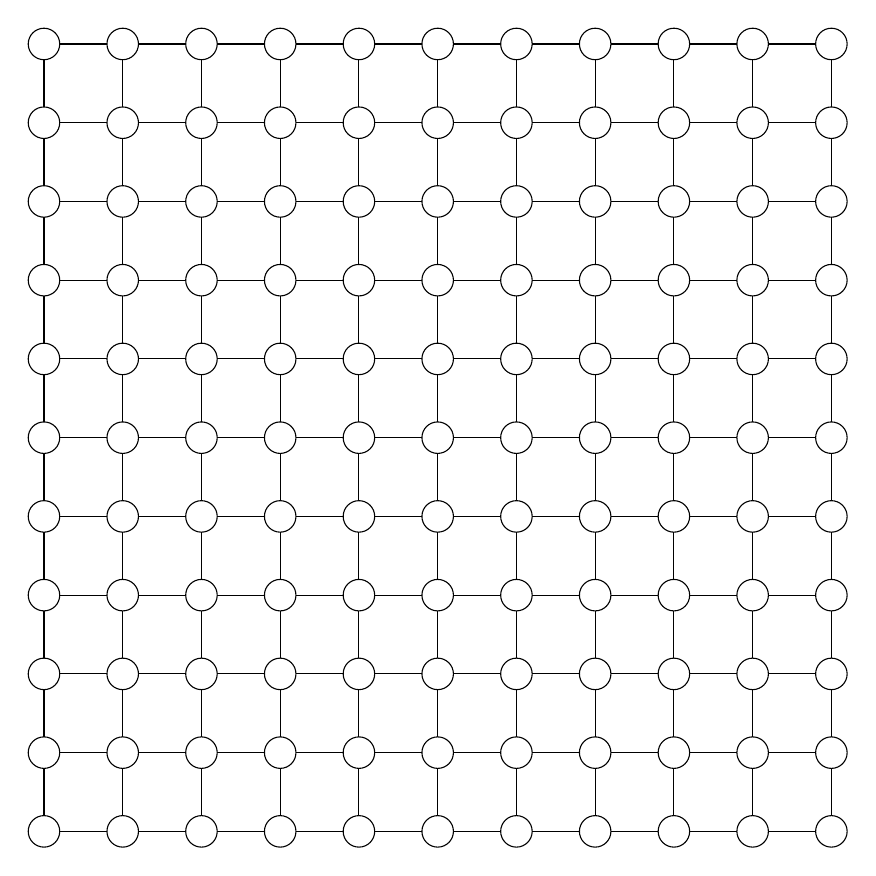
\begin{tikzpicture}

\foreach \x in {0,1,2,..., 10}
\foreach \y in {0,1,2,..., 10}
\draw (\x, \y) circle (0.2cm) ; 


\foreach \x in {0,1,2,..., 9}{
\foreach \y in {0,1,2,..., 10}{
\draw (\x+0.2, \y) -- (\x+0.8, \y) ;
}}

\foreach \x in {0,1,2,..., 10}{
\foreach \y in {0,1,2,..., 9}{
\draw (\x, \y+0.2) -- (\x, \y+0.8) ;
}}
\end{tikzpicture}
%\begin{figure}[h]
%\begin{center}
%
\includegraphics[width=.7\textwidth]{Imaging.png}
\caption{\label{fig:grid} Graph forming a two-dimensional regular
  grid.}
\end{center}
\end{figure}
The Ising model is moreover usually defined on a regular lattice,
which, in two dimensions, implies that $V$ is a finite
rectangle in $\mZ^2$, for example $V = \defset{-N,\ldots, N}^2$. The simplest
choice of a translation- and 90-degree rotation-invariant graph is the
nearest-neighbor graph for which $\defset{(i,j), (i',j')}\in E$ if and
only if $|i-i'| + |j-j'| =1$ (see \cref{fig:grid}). With this graph, one can furthermore
simplify the model to obtain the {\em isotropic Ising model} given by
$$
\pi(x) = \frac{1}{Z} \exp\Big( - \al \sum_{s\in V} \pe xs - \be
\sum_{s\sim t} \pe xs \pe xt\Big) .
$$
When $\be <0$, the model is {\em ferromagnetic}: each pair of
neighbors with identical signs brings a negative contribution to the
energy, making the configuration more likely (since lower energy
implies higher probability). 

The Potts model generalizes the Ising model  to finite, but non-necessarily binary, state spaces, say, $F_s
=F= \defset{1, \ldots, n}$. Define the function $\de(\la, \mu) = 1$ if
$\la=\mu$ and $(-1)$ otherwise. Then the Potts model is  given by
\begin{equation}
\label{eq:potts.model}
\pi(x) = \frac{1}{Z} \exp\Big( - \al \sum_{s\in V} h(\pe xs) - \be
\sum_{s\sim t} \de(\pe xs, \pe xt)\Big) 
\end{equation}
for some function $h$ defined on $F$.

\section{General state spaces}
\label{sec:mrf.pdf}

Our discussion of Markov random fields on graphs was done under the assumption of finite state spaces, which notably simplifies many of the arguments and avoids relying too much on measure theory. 
While this situation does cover a large range of application, there are cases in which one wants to consider variables taking values in continuous spaces, or in countable (infinite) spaces.

The results obtained for discrete variables can most of the time be extended to variables whose distribution has a p.d.f. with respect to a product of measures on the sets in which they take their values. For example, let $X, Y, Z$ takes values in $\CR_X, \CR_Y, \CR_Z$, equipped with $\sigma$-algebras $\boldsymbol{\CS}_X$, $\boldsymbol{\CS}_Y$, $\boldsymbol{\CS}_Z$ and measures $\mu_X$, $\mu_Y$, $\mu_Z$. Assume that $P_{X,Y,Z}$ is absolutely continuous with respect to $\mu_X\otimes \mu_Y\otimes \mu_Z$, with density $\phi_{XYZ}$. In such a situation, \cref{eq:cond.ind} remains valid, in that $X$ is conditionally independent of $Y$ given $Z$ if and only if
\begin{equation}
\label{eq:cond.ind.pdf}
\phi_{XYZ}(x,y,z) \phi_Z(z) = \phi_{XZ}(x,z) \phi_{YZ}(y,z)
\end{equation}
almost everywhere (relative to $\mu_X\otimes \mu_Y\otimes \mu_Z$). Here, $\phi_{XZ}, \phi_{YZ}, \phi_Z$ are marginal densities of the indexed random variables. The only difficulty in the argument, provided below for the interested reader, is dealing properly with sets of measure zero. 
\begin{proof}[Proof of \cref{eq:cond.ind.pdf}]
 Introduce the conditional densities
\[
\phi_{XY\mid Z}(x,y\mid z) = \frac{\phi_{XYZ}(x,y,z)}{\phi_Z(z)}
\]
and similarly $\phi_{X\mid Z}$ and $\phi_{Y\mid Z}$, which are defined when $z\not \in M_Z = \{z\in \CR_Z: \phi_Z(z) = 0\}$.  By definition of conditional independence, we have, for all $A \in \boldsymbol{\CS}_X$, $B\in \boldsymbol{\CS}_X$
\[
\int_{A\times B} \phi_{XY\mid Z}(x,y\mid z) \mu_X(dx)\mu_Y(dy) = 
\int_{A\times B} \phi_{X\mid Z}(x\mid z)\phi_{Y\mid Z}(y\mid z) \mu_X(dx)\mu_Y(dy) 
\]
for all $z\not \in M_Z$, which implies that, for all $z\not \in M_Z$, there exists a set $N_z\subset R_X\times R_Y$ such that $\mu_X\times \mu_Y(N_z) = 0$ and
\[
\phi_{XY\mid Z}(x,y\mid z) = \phi_{X\mid Z}(x\mid z)\phi_{Y\mid Z}(y\mid z)
\]
for all $z\not \in M_Z$ and $(x,y)\not \in N_z$. This immediately implies \cref{eq:cond.ind.pdf} for those $(x,y,z)$.  

If $z\in M_Z$, then 
\[
0 = \phi_Z(z) = \int_{\CR_X} \phi_{XZ}(x,z) \mu_X(dx) = \int_{\CR_Y} \phi_{YZ}(x,z) \mu_Y(dy)
\]
implying that $\phi_{XZ}(x,z) = \phi_{YZ}(y, z) = 0$  excepted on some set $N_z$ such that $\mu_{X}\otimes \mu_Y(N_z) = 0$, and \cref{eq:cond.ind.pdf} is therefore also true outside of this set. Now, letting $N = \{(x,y,z): (x,y) \in N_z\}$, we find that \cref{eq:cond.ind.pdf} is true for all $(x,y,z) \not \in N$ and
\[
\mu_X\otimes \mu_Y \otimes \mu_Z(N) = \int_{\CR_X\times \CR_Y\times \CR_Z} \bfone_{(x,y)\in N_z} \mu_X(dx)\mu_Y(dy)\mu_Z(dz) = \int_{\CR_Z}\mu_X\otimes \mu_Y(N_z)\mu_Z(dz) = 0.
\] 
(This argument involves Fubini's theorem \cite{rudin1966real}.)
\end{proof} 
With this definition, the proof of \cref{prop:cind} can be caried on without change, with the positivity condition expressing the fact that there exists $\tilde R_X \subset \CR_X$, $\tilde R_Y \subset \CR_Y$ and $\tilde R_Z \subset \CR_X$ such that $\phi_{XYZ}(x,y,z) > 0$ for all $x,y,z\in \tilde R_X \times \tilde R_Y \times \tilde R_Z$. (This proposition is actually valid in full generality, with a proper definition of positivity.)


When considering random fields with general state spaces, we will restrict to the similar situation in which each state space $F_s$ is equipped with a $\sigma$-algebra $\boldsymbol{\CS}_s$ and a measure $\mu_s$, and the joint distribution, $P_X$ of the random field $X  = (X_s, s\in V)$  is absolutely continuous with respect to $\mu\defeq \bigotimes_{s\in V} \mu_s$, denoting by $\pi$ the corresponding p.d.f. We will says that $\pi$ is positive if there exists $\tilde F = (\tilde F_s, s\in V)$ with measurable $\tilde F_s \subset F_s$ such that $\pi(x) > 0$ for all $x\in \CF(V, \tilde F)$. Without loss of generality unless one considers multiple random fields with different supports, we will assume that $\tilde F_s = F_s$ for all $s$.


The definition of consistent families of local interactions (\cref{def:set.int}) must be modified by adding the condition that
\begin{equation}
\label{eq:local.int.bounded}
\int_{\CF(V)} \prod_{C\in \CC}\phi_C(\pe x C) \mu(dx) < \infty.
\end{equation}
This requirement is obviously needed to ensure that the normalizing constant in \cref{eq:pi.phi} is finite. \Cref{prop:gc} is then true (with sums replaced by integrals in the proof) and so are \cref{prop:gc.cond,prop:gc.m}. Finally, the Hammersley-Clifford theorem (\cref{th:ham.clif.1}) extends to this context.

Even though it is a natural requirement, condition \eqref{eq:local.int.bounded} may be hard to assess with general families of local interactions. In the case of Gaussian distributions, however, one can provide relatively simple conditions. Assume that $F_s = \mR$ for all $s\in V$, and condider a potential $\Lambda = (\lambda_C, C\in \CC)$ with only univariate and bivariate interactions, such that, for some vector $a\in \mR^d$ (with $d = |V|$) and symmetric matrix $b \in \CS_d$,
\[
\left\{
\begin{aligned}
\lambda_{\{s\}}(\pe x {\{s\}}) &= -\pe as \pe xs + \frac12 b_{ss} (\pe xs)^2\\
\lambda_{\{s,t\}}(\pe x {\{s,t\}}) &=  b_{st} \pe xs\pe xt
\end{aligned}
\right.
\]
Then, considering $x\in \CF(V)$ as a $d$-dimensional vector, we have
\[
\pi(x) = \frac{1}{Z} \exp\left(a^T x - \frac12 x^T b x\right),
\]
with the integrability requirement that $b \succ 0$ (positive definite). The random field then follows a Gaussian distribution with mean $m = b^{-1} a$ and covariance matrix $\Sigma = b^{-1}$. The normalizing constant, $Z$, is given by
\[
Z = \frac{e^{-\frac12 a^Tba}(2\pi)^{d/2}}{\sqrt{\det{b}}}.
\]


This Markov random field parametrization of Gaussian distributions emphasizes the conditional  structure of the variables rather than their covariances. It is useful when the associated graph, represented by the matrix $b$ is sparse. In particular, the conditional distribution of $\pe Xs$ given the other variables is Gaussian, with mean $(\pe a s - \sum_{t\neq s} b_{st} \pe x t)/b_{ss}$ and variance $1/b_{ss}$.













%
%
%
%The notion of positivity of the joint density of random variables $X_1, \ldots, X_N$ taking values in measures sets $(R_{X_k}, \boldsymbol{\CS}_k, k=1, \ldots, N)$ just states that
%\[
%\myP(X_1\in A_1, \ldots, X_N\in A_N) = 0 \Ria \exists k\in\{1, \ldots, N\}:
%\myP(X_k\in A_k) = 0.
%\]
%With this definition \cref{prop:cind} remains valid. One can then proceed to a general definition of Markov random fields for arbitrary variables. 
%
% 
%
%We first prove a consequence of \cref{eq:cond.ind.gen}
%\begin{proposition}
%\label{prop:cond.ind.gen} Let $X, Y, Z$ taking values into measurable spaces $R_X, R_Y, R_Z$.
%One has $(X\indp Y \mid Z)$ if and only if, for all measurable functions $f: R_X \to \mR$:
%\begin{equation}
%\label{eq:cond.ind.gen.3}
%E(f(X)\mid Y, Z) = E(f(X)\mid Z)
%\end{equation}
%\end{proposition}
%\begin{proof} 
%
%Assume \cref{eq:cond.ind.gen}.
%Then, for any functions $g: R_Y \to\mR$, $h: R_Z\to \mR$
%\[
%\myE(f(X)g(Y)h(Z)) = \myE(\myE(f(X) g(Y)\mid Z) h(Z)) = \myE(\myE(f(X) \mid Z) \myE(g(Y)\mid Z) h(Z))  = \myE(\myE(f(X) \mid Z) \myE(g(Y)h(Z)\mid Z))  = \myE(\myE(f(X) \mid Z) g(Y) h(Z)).
%\]
%So, we have
%\[
%\myE(f(X)a(Y, Z)) = \myE(\myE(f(X) \mid Z) a(Y,Z))
%\]
%for all function $a: R_Y \times R_Z \to \mR$ that split into a product of two functions. This remains true for sums of such functions and then for all functions $a$ by density. 
%
%Conversely, assuming \cref{eq:cond.ind.gen.3}, we have 
%\[
%\myE(f(X)g(Y)h(Z)) = \myE(\myE(f(X)\mid Y,Z) f(Y) h(Z)) = \myE(\myE(f(X)\mid Z) f(Y) h(Z)) = \myE(\myE(f(X)\mid Z) \myE(f(Y)\mid Z) h(Z)),
%\]
%which yields \cref{eq:cond.ing.gen.1}
%\end{proof}
%\Cref{eq:cond.ing.gen} implies the the seemingly more general fact that
%\begin{equation}
%\label{eq:cond.ind.gen.2}
%\myE(f(X, Z)g(Y, Z)\mid Z) = \myE(f(X, Z)\mid Z)\myE(g(Y, Z)\mid Z).
%\end{equation}
%
%To show this, first checks that this holds when $f(x,z)=f_1(x)f_2(z)$ and
%$g(y,z)=g_1(y)g_2(z)$ since in this case
%\[
%\myE(f(X)g(Y)\mid Z) = f_2(Z) g_2(Z)  \myE(f_1(X)g_1(Y)\mid Z),
%\]
%in which case \cref{eq:cond.ind.gen.2} is a consequence of \cref{eq:cond.ind.gen}. By linearity, \cref{eq:cond.ind.gen.2} is also true for linear combinations of such functions and the result follows by a density argument. 



% !TeX root = graphical.tex

% !TeX root = graphical.tex

